\documentclass[a4paper,12pt]{Latex/Classes/PhDthesisPSnPDF}
\usepackage[utf8]{inputenc}
\usepackage{amsthm}
\usepackage{graphicx}
\usepackage{siunitx, booktabs}
\usepackage{caption}
\setlength{\parindent}{4em}
\setlength{\parskip}{1em}

% \usepackage[spanish]{babel}
% \input{body/preamble/preamble.Rnw}
% This file contains macros that can be called up from connected TeX files
% It helps to summarise repeated code, e.g. figure insertion (see below).

%%%%%%%%%%%%%%%%%%%%%%%%%%%%%%%%%%%%%%%%%%%%%%
%            Colores de la UNAM              %
%%%%%%%%%%%%%%%%%%%%%%%%%%%%%%%%%%%%%%%%%%%%%%
%Azul Pantone 541  -->(0,63,119) RGB
\definecolor{Azul}{RGB}{128,0,0}

%Oro Pantone 460  -->(234,221,150) RGB
\definecolor{Oro}{RGB}{234,221,150}


%%%%%%%%%%%%%%%%%%%%%%%%%%%%%%%%%%%%%%%%%%%%%%
%            Comandos para líneas            %
%%%%%%%%%%%%%%%%%%%%%%%%%%%%%%%%%%%%%%%%%%%%%%
%Se define un comando \colorvrule para hacer líneas verticales de color con 3 argumentos: color, ancho, alto
\newcommand{\colorvrule}[3]{
\begingroup\color{#1}\vrule width#2 height#3
\endgroup}

%Se define un comando \colorhrule para hacer líneas horizontales de color con 2 argumentos: color, ancho
\newcommand{\colorhrule}[2]{
\begingroup\color{#1}\hrule height#2
\endgroup}

%%%%%%%%%%%%%%%%%%%%%%%%%%%%%%%%%%%%%%%%%%%%%%
%          Comando para derivadas            %
%%%%%%%%%%%%%%%%%%%%%%%%%%%%%%%%%%%%%%%%%%%%%%
\newcommand{\derivada}[3][]{\ensuremath{\dfrac{\mbox{d}^{#1}#2}{\mbox{d}#3^{#1}}}} 
%primer argumento(opcional): orden de la derivada
%segundo argumento: función a derivar
%tercer argumento: variable respecto a la que se deriva


%%%%%%%%%%%%%%%%%%%%%%%%%%%%%%%%%%%%%%%%%%%%%%
%       Comando para la exponencial          %
%%%%%%%%%%%%%%%%%%%%%%%%%%%%%%%%%%%%%%%%%%%%%%
\newcommand{\e}[1][]{\ensuremath{\mbox{e}^{#1}}}
%primer argumento(opcional): exponente de la exponencial




% insert a centered figure with caption and description
% parameters 1:filename, 2:title, 3:description and label
\newcommand{\figuremacro}[3]{
	\begin{figure}[htbp]
		\centering
		\includegraphics[width=1\textwidth]{#1}
		\caption[#2]{\textbf{#2} - #3}
		\label{condicion}
	\end{figure}
}

% insert a centered figure with caption and description AND WIDTH
% parameters 1:filename, 2:title, 3:description and label, 4: textwidth
% textwidth 1 means as text, 0.5 means half the width of the text
\newcommand{\figuremacroW}[4]{
	\begin{figure}[htbp]
		\centering
		\includegraphics[width=#4\textwidth]{#1}
		\caption[#2]{\textbf{#2} - #3}
		\label{#1}
	\end{figure}
}

% inserts a figure with wrapped around text; only suitable for NARROW figs
% o is for outside on a double paged document; others: l, r, i(inside)
% text and figure will each be half of the document width
% note: long captions often crash with adjacent content; take care
% in general: above 2 macro produce more reliable layout
\newcommand{\figuremacroN}[3]{
	\begin{wrapfigure}{o}{0.5\textwidth}
		\centering
		\includegraphics[width=0.48\textwidth]{#1}
		\caption[#2]{{\small\textbf{#2} - #3}}
		\label{#1}
	\end{wrapfigure}
}

% predefined commands by Harish
\newcommand{\PdfPsText}[2]{
  \ifpdf
     #1
  \else
     #2
  \fi
}

\newcommand{\IncludeGraphicsH}[3]{
  \PdfPsText{\includegraphics[height=#2]{#1}}{\includegraphics[bb = #3, height=#2]{#1}}
}

\newcommand{\IncludeGraphicsW}[3]{
  \PdfPsText{\includegraphics[width=#2]{#1}}{\includegraphics[bb = #3, width=#2]{#1}}
}

\newcommand{\InsertFig}[3]{
  \begin{figure}[!htbp]
    \begin{center}
      \leavevmode
      #1
      \caption{#2}
      \label{#3}
    \end{center}
  \end{figure}
}







%%% Local Variables:
%%% mode: latex
%%% TeX-master: "~/Documents/LaTeX/CUEDThesisPSnPDF/thesis"
%%% End:
 
\newtheorem{teorema}{Teorema}
\newtheorem{definicion}{Definición}
% \showboxdepth=5
% \showboxbreadth=5
%%%%%%%%%%%%%%%%%%%%%%%%%%%%%%%%%%%%%%%%%%%%%%%%%%%%%%%%%%%%%%%%%%%%%%%%%%%%%%%%
%                                   DATOS                                      %
%%%%%%%%%%%%%%%%%%%%%%%%%%%%%%%%%%%%%%%%%%%%%%%%%%%%%%%%%%%%%%%%%%%%%%%%%%%%%%%%
\title{Evaluación de la Eficacia de una estrategia de trading basada en Modelo Lineal Generalizado}
\author{Rodrigo Alejandro Serrano Morales} 
\facultad{Facultad de Ciencias Económicas y Sociales\\
Escuela de Estadística y Ciencias Actuariales}                % Nombre de la facultad/escuela
\escudofacultad{images/faces} % Aquí ponen la ruta y nombre del escudo de su facultad, actualmente, la carpeta Latex/Classes/Escudos cuenta con los siguientes escudos:
% "fi_azul" Facultad de ingenieria en color azul
% "fi_negro" Facultad de ingenieria en color negro
% "fc_azul" Facultad de ciencias en color azul
% "fc_negro" Facultad de ciencias en color negro
% Se agradecen sus aportaciones de escudos a jebus.velazquez@gmail.com

\degree{Licenciado en Ciencias Actuariales}        % Carrera
\director{Prof. Jonattan Ramos \& Prof. Eloy Eligon}               % Director de tesis
\degreedate{Marzo 2019}                           % Año de la fecha del examen
\lugar{Caracas}                        % Lugar

%\portadafalse                              % Portada en NEGRO, descomentar y comentar la línea siguiente si se quiere utilizar
\portadatrue                                % Portada en COLOR



%% Opciones del posgrado (descomentar si las necesitan)
	%\posgradotrue                                                    
	%\programa{programa de maestría y doctorado en ingeniería}
	%\campo{Ingeniería Eléctrica - Control}
	%% En caso de que haya comité tutor
	%\comitetrue
	%\ctutoruno{Dr. Emmet L. Brown}
	%\ctutordos{Dr. El Doctor}
%% Datos del jurado                             
	%\presidente{Dr. 1}
	%\secretario{Dr. 2}
	%\vocal{Dr. 3}
	%\supuno{Dr. 4}
	%\supdos{Dr. 5}
	%\institucion{el Instituto de Ingeniería, UNAM}

\keywords{tesis,autor,tutor,etc}            % Palablas clave para los metadatos del PDF
\subject{tema_1,tema_2}                     % Tema para metadatos del PDF  

%%%%%%%%%%%%%%%%%%%%%%%%%%%%%%%%%%%%%%%%%%%%%%%%%%%%%
%                   PORTADA                         %
%%%%%%%%%%%%%%%%%%%%%%%%%%%%%%%%%%%%%%%%%%%%%%%%%%%%%
\usepackage{Sweave}
\begin{document}
\Sconcordance{concordance:main.tex:main.Rnw:%
1 64 1 1 0 14 1}
\Sconcordance{concordance:main.tex:./body/introduccion/introduccion.Rnw:ofs 80:%
1 11 1}
\Sconcordance{concordance:main.tex:./body/chapter1/chapter1.Rnw:ofs 92:%
1 43 1}
\Sconcordance{concordance:main.tex:./body/chapter2/chapter2.Rnw:ofs 136:%
1 255 1 1 18 1 2 17 1}
\Sconcordance{concordance:main.tex:./body/chapter3/chapter3.Rnw:ofs 411:%
1 95 1 1 64 3 1 2 2 32 1}
\Sconcordance{concordance:main.tex:./body/chapter4/chapter4.Rnw:ofs 545:%
1 15 1 1 14 3 1 2 2 13 1 1 8 1 3 7 1 1 8 1 2 4 1 1 74 2 1 1 3 1 2 8 1 1 %
3 1 2 8 1 1 3 1 2 8 1 1 12 5 1 1 9 1 2 12 1 1 14 1 2 9 1 1 3 1 2 13 1 1 %
7 1 2 4 1 1 7 3 1 1 7 1 2 22 1 1 3 9 0 1 2 1 1 1 32 1 2 8 0 1 1 7 0 1 2 %
9 0 1 1 10 0 1 2 12 1 1 7 12 0 1 2 3 1 1 6 12 0 1 2 3 1 1 6 12 0 1 2 4 %
1 1 6 12 0 1 2 3 1 1 6 12 0 1 2 4 1 1 6 12 0 1 2 7 1 1 37 2 1 1 2 15 0 %
1 2 3 1 1 26 5 1 1 9 1 2 4 1 1 24 3 1 1 9 1 2 15 1 1 17 2 1 1 2 14 0 1 %
2 3 1 1 27 2 1 1 2 11 0 1 2 2 1}
\Sconcordance{concordance:main.tex:./body/conclusion/conclusion.Rnw:ofs 976:%
1 7 1 1 20 3 1 1 6 1 2 15 1}
\Sconcordance{concordance:main.tex:./body/anexos/anexos.Rnw:ofs 1005:%
1 9 1 1 2 12 0 1 2 3 1 1 2 12 0 1 2 2 1 1 2 12 0 1 2 5 1 1 2 12 0 1 2 3 %
1 1 2 12 0 1 2 2 1 1 2 12 0 1 2 6 1 1 2 12 0 1 2 3 1 1 2 12 0 1 2 3 1 1 %
2 12 0 1 2 5 1 1 2 12 0 1 2 3 1 1 2 12 0 1 2 2 1 1 2 12 0 1 2 6 1 1 2 %
12 0 1 2 3 1 1 2 12 0 1 2 2 1 1 2 12 0 1 2 5 1 1 2 12 0 1 2 3 1 1 2 12 %
0 1 2 2 1 1 2 12 0 1 2 6 1 1 2 12 0 1 2 4 1 1 2 12 0 1 2 2 1 1 2 12 0 1 %
2 5 1 1 2 12 0 1 2 3 1 1 2 12 0 1 2 2 1 1 2 12 0 1 2 1 1}
\Sconcordance{concordance:main.tex:./body/bibliografia/bibliografia.Rnw:ofs 1432:%
1 37 1}
\Sconcordance{concordance:main.tex:main.Rnw:ofs 1470:%
88 1 1}


\maketitle									% Se redefinió este comando en el archivo de la clase para generar automáticamente la portada a partir de los datos

\newpage\renewcommand{\thepage}{\arabic{page}}\setcounter{page}{1} 

% \SweaveInput{body/reconocimiento/reconocimiento.Rnw}
% \SweaveInput{body/agradecimientos/agradecimientos.Rnw}

\tableofcontents
\listoffigures
\listoftables


% !TeX root = ./main.Rnw
%\SweaveUTF8

\chapter*{Introducción}
\addcontentsline{toc}{chapter}{Introduccion}

Las economías de países latinoamericanos son reconocidas históricamente por depender en gran magnitud del comercio de sus materias primas, lo cual hace que el comercio con dichos commodities resulte de gran impacto para el gasto fiscal y para la balanza de pagos, esto deja como consecuencia, la necesidad de los actores económicos de estudiar el riesgo a profundidad para poder evitar resultados que reduzcan sus retornos positivos.\\ 

% !TeX root = ./main.Rnw
%\SweaveUTF8

\chapter{El Problema}

\section{Justificación}

A principios del siglo XX los mercados bursátiles eran operados manualmente, los corredores y demás participantes realizaban una serie de labores sin asistencia de sistemas informáticos, que evidentemente no existían para la época. El 8 de febrero de 1971 comienza operaciones la bolsa de valores NASDAQ -National Association of Securities Dealers Automated Quotation-, la cual marca un precedente en la industria. NASDAQ fue el primer mercado bursátil en el mundo en adoptar el uso de sistemas electrónicos para proveer cotizaciones de las acciones. Más tarde añadirían, también, la capacidad de manejar operaciones electrónicamente, ejecutando órdenes de compras y ventas sin necesidad de encontrarse físicamente en el lugar destinado para las transacciones.

Este precedente aunado con el rápido crecimiento de la industria tecnológica y la creación del internet, facilitan al mercado bursátil digitalizarse rápidamente. Esto permite a los competidores y la industria en general obtener un sistema más eficiente en términos de operatividad, además de globalizar la actividad financiera y propiciar la participación de más inversores en los mercados. El globalizar la información incrementa la competitividad en el sector e incentiva estudios de privados e independientes para maximizar retornos, de donde surgen los análisis técnicos y fundamentales.

Ahora bien la iniciación al mundo bursátil trae consigo grandes riesgos si no se opera con conocimiento y planificación financiera. Es por esto que cada año los individuos pierden dinero al querer incursionar en el mundo del trading sin la preparación adecuada, lo que por otro lado, le da oportunidad a participantes ya establecidos y con conocimiento de aprovechar esta dinámica. El trading requiere de una planificación exhaustiva en cuanto al manejo de riesgo y aplicación de estrategias, es así como los algoritmos automáticos suponen un manejo ideal de los factores, estableciendo reglas sistemáticas para las operaciones.

En los últimos años y con el impulso de computadores cada vez más potentes, ha surgido un nicho dentro del mercado financiero destinado a compañías que operan con algoritmos automatizados, llamadas comúnmente “Quantitave Funds” -Fondos Cuantitativos-. Según un informe realizado por Credit Suisse Group, estos fondos son los de mayor crecimientos en los últimos años. Los fondos cuantitativos y de inversión pasiva controlan actualmente el 60\% de los activos del mercado, incluso, tan solo el 10\% del volumen de transacciones proviene de inversores discrecionales, según JPMorgan Chase \& Co. en cita de Bloomberg. Es así como compañías como Goldman Sachs han reemplazado gran cantidad de operadores por algoritmos, como dio a conocer en el 2017. La mayoría de las grandes instituciones y proveedores del sector ya cuentan con servicios que cumplen con los requerimientos para la aplicación de los sistemas automatizados, como plataformas con puertos API y datas históricas destinadas a testear algoritmos de trading. En palabras de Frank Thermitus (2018), presidente de la Asociación de Trading Algorítmico de Argentina “No tenemos datos oficiales en Argentina, pero sabemos que la aparición de soporte para este tipo de trading está llamando a un crecimiento de la participación de agentes automatizados”.

La mayor ventaja del trading basado en algoritmos es que realiza la labor de inversión de manera sistemática, removiendo el factor emocional de las personas. Apegarse a un estrategia de inverión es vital para lograr resultados consistentes en el trading. Sin embargo, es difícil encontrar estrategias que generen rendimientos positivos todo el tiempo, y aún así los factores emocionales de las personas pueden destruir cualquier plan al enfrentarse a momentos transitorios de pérdida continua, llamados 'drawdowns' en el mundo financiero. El necesitar un plan consistente y sistemático, promueve la utilización de sistemas automatizados dado que elimina cualquier aspecto emocional durante el proceso de la inversión, manteniendo la disciplina durante momentos de alta volatilidad.

La otra gran ventaja de los sistemas automatizados es que permite la posibilidad de realizar pruebas del algoritmo en data histórica para entender el comportamiento de la estrategia, este proceso es conocido como 'backtesting'. De esta manera el inversor tiene una idea de como se comportará el sistema en situaciones similares a las testeadas en el backtesting. El backtesting también permite optimizar los parámetros de la estrategia en busca de máximizar los retornos con el menor riesgo, sin embargo, se debe tener cuidado en no sobreoptimizar el sistema. 

\section{Planteamiento del Problema}

Con este panorama es evidente la utilidad que supone la utilización de métodos de aprendizaje estadístico para el desarrollo de algoritmos automáticos. El aprendizaje estadístico, referido en la literatura anglosajona como “Machine Learning” es definido por uno de sus principales exponentes -el profesor de la universidad de Carnegie Mellon- Tom Mitchell como “el campo de estudio que da a las computadoras la habilidad de aprender sin ser explícitamente programada”. En este sentido, expone que “Un algoritmo aprende de la experiencia E con respecto a una tarea T cuyo rendimiento es medido por el indicador P, si su desempeño en T como medida de P mejora con la experiencia E”. Esta referencia a que la “computadora aprende”, no son más que técnicas estadísticas aplicadas a distintos problemas, en donde se busca mejorar el desempeño del modelo calibrando una medida de error.

El desarrollo tecnológico, especialmente el potenciamiento de los procesadores computacionales y el surgimiento del software libre, han provocado un crecimiento en el número de profesionales que aplican el “Machine Learning”. Esto ha ocasionado que innumerables problemas sean abordados con estas técnicas, desde transformar historiales de compras de consumidores en enfoques publicitario, ó intentar imitar el razonamiento humano en una tarea en específico, como jugar ajedrez.

En la presente investigación se busca utilizar las técnicas de aprendizaje estadístico para realizar predicciones sobre el comportamiento de un activo financiero en el corto  plazo, intentando capitalizar este conocimiento. Ahora bien, existe un debate sobre si las inversiones activas, son realmente efectivas. La principal razón de la polémica, es debido a la complejidad que involucra realizar una predicción con tan poco margen de error y durante un período de tiempo sostenido. Aunado de las múltiples fuentes de riesgo concernientes a los portafolios de inversión, sería impensable tratar de definir en una primera investigación una estrategia eficaz para el desarrollo del trading.

Por otro lado el explosivo crecimiento en los últimos años de los métodos de aprendizaje estadístico ha creado innumerables variantes de los algoritmos, por lo que abarcar varios de estos supondría un trabajo arduo, realizado probablemente por un equipo de trabajo con experiencia, tanto en el mundo financiero como computacional y estadístico. En las investigaciones similares a la presente, se toman algunos métodos y se intenta definir cuáles de ellos arroja mayor precisión. En esta investigación se abordará el aprendizaje supervisado, basado en un modelo lineal generalizado -MLG-, específicamente, una regresión logística. Se intenta contrarrestar la debilidad de asumir linealidad en el modelo, agrupando las variables con una técnica no supervisada como el Análisis de Componentes Principales.

La idea del modelo es predecir los casos en los cuales, el incurrir en una posición en largo provocaría una ganancia, asegurando que la posición se capitalice a un porcentaje t del precio inicial, sin antes haber incurrido en una pérdida de s porciento, en un horizonte de tiempo h. Es decir que en el intervalo de tiempo h debe ocurrir primero la toma de ganancia -take profit- que la pérdida -stop loss-. Para esto se identifica en un período de la data utilizada, todas las observaciones en la que esto ocurre, y se intenta generar un modelo que entienda las condiciones del activo cuando este patrón sucede.

\section{Objetivo General}

Evaluar la eficacia de una estrategia de trading basada en técnicas de aprendizaje estadístico

\section{Objetivos Específicos}

\begin{itemize}
\item Definir los parámetros de la estrategia, así como los indicadores técnicos a utilizar como variables predictoras
\item Utilizar Análisis de Componentes Principales como técnica de reducción de la dimensión de variables predictoras
\item Aplicar Regresión Logística con las componentes arrojadas por el ACP
\item Desarrollar la metodología Walkforward para tomar en cuenta el dinamismo del mercado en la estrategia
\item Evaluar la predicción del modelo como estrategia en los índices seleccionados
\end{itemize}

% !TeX root = ./main.Rnw
%\SweaveUTF8

\chapter{Marco Teórico}

\section{Antecedentes}

\subsection{Trading de Cryptomonedas basado en Aprendizaje Automatico}

Bach y Nielsen examinan la efectividad de diversos algoritmos de aprendizaje estadístico para operar en el mercado de cryptomonedas. Establecen un marco de trabajo en lenguaje R que les permite probar los distintos algoritmos cambiando las variables predictoras. Utilizan diversos intervalos de tiempo desde 1 minuto hasta 24 horas, diversos indicadores como ADX, MACD y RSI, así como algunas asociaciones establecidas manualmente. Consideraron cuatro algoritmos: Regresión Logística, Redes Neuronales, Gradient Boosting y Bosques aleatorios. Utilizan el mismo enfoque en cuanto a buscar predecir la subida del precio dado un objetivo sin salir por 'Stop Loss' en un determinado período de tiempo.

\subsection{Un enfoque de aprendizaje automático para el comercio automatizado}

Ning Lu explora la aplicación de varios algoritmos de aprendizaje enfocados en el trading automático, entre ellos: Regresión Logística, Naïve Bayes y Máquinas de vectores de soporte. Los algoritmos son probados en activos pertenecientes al S\&P500. El enfoque de Lu es el de utilizar como variables predictoras no solo precios del activo en el cual se va a invertir, sino, usar información de precios de otros activos que puedan influir en el activo principal.

\subsection{Modelos predictivos para el mercado FOREX}

Huerta López utiliza dos enfoques para el trading automático en el mercado FOREX: los modelos de series de tiempo y los modelos basados en técnicas de aprendizaje automático. Por un lado aplica modelos ARIMA y métodos de automatización para su implementación basados en criterios de información -BIC y AIC-. Para el enfoque basado en aprendizaje automático implementa diversos algoritmos de KNN y Árboles de desición, optimizando los algoritmos en la distintas horas del día utilizando datos del par EUR-USD. Señala que los modelos de aprendizaje obtienen mejor predicción que los modelos ARIMA, acercandose a un 60\% de precisión.

\subsection{Un Análisis de estrategias de trading técnico}

Kadida Shagilla profundiza sobre las alternativas a la hipótesis del mercado eficiente y como se relacionan el riesgo y los retornos de una estrategia de trading. Simula tres portafolios conformados por una muestra de acciones de tres mercados Norteamericanos y algunos mercados emergentes de Africa. El estudio demuestra como la relación 'book-to-market ratio', la liquidez y los acuerdos institucionales pueden explicar el exceso de ganancia a partir del análisis técnico. 

\subsection{Modelos Ocultos de Markov Aplicados al Reconocimiento de Patrones del Análisis Técnico Bursátil}

Cristián Fernández introduce un sistema autómatico para el reconocimiento de patrones del análisis técnico basado en modelos de Markov. Desarrolla un algoritmo que extrae patrones del mercado y los clasifica en tres estados: lateral, alcista y bajista. Utiliza una clasificación basada en Árboles de desición y apoya el reconocimiento de patrones en algunos indicadores técnicos. Concluye que es posible estimar correctamente el estado de un activo mediante una lectura automática de los patrones en su serie de tiempo. El modelo es testeado en varios activos que operan en el mercado bursátil argentino.


\section{Bases Teóricas}


\subsection{Hipótesis del Mercado Eficiente}

La Hipótesis del Mercado eficiente fue desarrollada por Eugene Fama en los años 60, en la misma argumenta que los precios de los activos reflejan toda la información disponible, es decir que siempre son transados a un valor adecuado para su riesgo, haciendo imposible para los inversores obtener retornos más elevados que los del mercado en general. 

Fama sugiere tres suposiciones. Primero, el mercado eficiente requiere un gran número de competidores buscando maximizar ganancias. Segundo, la información que afecta al activo llega al mercado de manera aleatoria y cada anuncio es independiente de los demás. Tercero, todos los competirdores intentarán ajustar sus posiciones lo más rapido posible conocida la información del mercado. Existen tres variantes de la hipótesis:

Eficiencia débil, en esta variante, los precios del pasado no sirven para predecir el precio futuro, es decir cualquier movimiento del activo es determinado por información no contenida en la serie de precios. Eficiencia media, en esta forma se asume que los precios se ajustan instantáneamente a la información pública, por lo que rechaza cualquier tipo de arbitraje intentando aprovechar nueva información. Eficiencia fuerte, esta última forma de la hipótesis plantea que los precios reflejan tanto información pública como privada, por lo cual incluso obteniendo información no conocida por todos los competidores, no se pueden obtener retornos anormales al de los mercados.

Aunque esta hipótesis es la piedra angular de la teoría financiera moderna, es controversial entre la comunidad financiera y dispustada frecuentemente. Gran parte de sus detractores argumentan que el precio del activo está influenciado por suposiciones cesgada de los individuos, formuladas por la manera en como estos responden ante nueva información.

Los inversores interpretan la información de manera distinta, por lo que generarán diferentes valuaciones de un mismo activo, lo que sugiere que la reacción del inversor a la misma noticia será distinta. Day and Wangr (2002) argumentan que si los precios son continuamente influenciados por estas interpretaciones erróneas, los movimientos contrarios del precio pueden ser predecidos estudiando la data histórica. Sugieren también que mientras más extremo sea el movimiento incial, mayor será el ajuste de precio.

Los inversores se dejan influenciar por la tendencia del mercado, este comportamiento se ha visto a lo largo de la historia en casos de colapso del mercado como en la caída del mercado búrsatil en 1987 ó la burbuja del puntocom a finales de los 90. Froot (1992) muestra como estos comportamientos pueden resultar en ineficiencias del mercado.

Aglunos académicos como Hong y Stein's (1999) categorizan a los inversores en $Informados$ y $No informados$. Los inversores que tienen acceso a la información solo operan al obtener nueva información, mientras que los no informados operan basados en el pasado reciente del activo. A medida que la información es conocida por todos los competidores, se forma el fenómeno de reversión a la media.

Es evidente la postura que se asume en la presente investigación con respecto a la hipótesis de mercado eficiente. Además de los aspectos del comportamiento de los competires, se ha evidenciado en la historia, casos de inversores que han logrado vencer el mercado por largos períodos de tiempo, como Warren Buffet, lo cual por definición de la hipótesis es imposible. Por otro lado, Los avances técnologicos y la capacidad de procesamiento de las computadoras en la actualidad hacen pensar que cualquier anomalía presente en el mercado por muy pequeña que sea puede ser aprovechada por sofisticados softwares automatizados. Shagilla Kadida (2006)

\subsection{Análisis Técnico}

Los inversionistas que rechazan la hipótesis del mercado eficiente buscan interpretar la situación del mercado, bien a través de noticias que afecten al activo o estudiando su movimiento intentando extrer patrones de conducta. A la primera técnica se le llama Análisis Fundamental y el segundo Análisis Técnico. El Análisis Fundamental está mas asociado a estrategias de inversión pasivas a largo plazo aunque en la actualidad se han desarrollado algoritmos de compra y venta que buscan predecir la dirección del precio en función de noticas utilizando minería de texto.

El análisis técnico es aquel que busca patrones y tendencias de comportamiento en la cotización de los activos financieros, basándose en la serie de tiempo del activo, con esto intenta predecir el movimiento futuro mediante el uso de gráficos. Según J.J.Murphy (1999) existen tres fundamentos básicos en los que se basa el análisis técnico: Los movimientos del mercado lo descuentan  todo, los precios se mueven por tendencias y la historia se repite.

Murphy establece que cualquier efecto que posiblemente pueda afectar al precio se ve reflejado en la cotización del mismo. Por lo que un estudio del desplazamiento del activo en un período de tiempo sería suficiente para lograr predecir su movimiento. Esto quiere decir que el análisis técnico no es mas que una manera indirecta de estudiar los fundamentos del activo, suponiendo que la cotización del mismo resume toda la información que lo afecta. 

El análista técnico acepta la premisa de que los mercados tienen tendencias. Buscar tendencias en las primeras etapas de su desarrollo es la razón de toda la representación gráfica dentro del análisis, con el fin de que las transacciones vayan en dirección de esa tendencia. Por otro lado, la afirmación de que la historia se repite tiene que ver con el estudio de la psicología humana. Ésta afirmación tiene también una estrecha relación en los ciclos económicos. 

A continuación se establece la formulación de cada indicador utilizado en el estudio, se utilizará la notación $EMA_{(t, p)}(X)$ para referirse a una media móvil exponencial en t calculada con p observaciones enteriores con respecto a la serie de precio X:

\begin{itemize}
\item Retornos con respecto al precio de Cierre.

$$ R_{t} = \frac{Pcierre_{t}}{Pcierre_{t-1}-1}$$

\item RSI (Relative Strength Index) de 14 períodos, el cual es un indicador de volatilidad.

$$ RSI_{t} = 100 - \frac{100}{1 + RS_{t}} \qquad 
donde, RS_{t} = \frac{Ganancia\ Promedio\ en\ n\ observaciones}{Pérdida\ Promedio\ en\ n\ observaciones}$$

\item MACD (Moving Average Converge/Divergence) el cual es una diferencia de dos EMAs (Exponential Moving Average) de 12 y 26 períodos. Este es un indicador de tendencia que se complementa con un MA(Moving Averge) de 9 períodos. 

$$ MACD_{t} =  EMA_{(t, 12)}(Pcierre) - EMA_{(t, 26)}(Pcierre) \qquad
Signal\ Line_{t} = EMA_{(t, 9)}(MACD_{t}) $$

\item ATR (Average True Range), es un indicador de volatilidad calculado a partir de los máximos y mínimos de un período, en este caso 14.

$$ ATR_{t} =  EMA_{(t, 14)}(TR_{t}) \qquad
TR_{t} = Max\ (Pmax - Pmin, |Pmax - Pc_{t-1}|, |Pmin - Pc_{t-1}|)$$

\item ADX (Average Directional Index), este es un indicador que utiliza dos indicadores de dirección +Di y -Di, se calculó en base a 14 períodos y mide tendencia.

$$ ADX_{t} =  100\ EMA_{(t, 14)}(|+DI - -DI|)$$

\item Bandas de Bollinger, el cual es un indicador de tendencia y volatilidad, utiliza dos bandas calculadas a partir de una media movil con desviaciones estándar. Se utilizó en base a 14 períodos y una desviación de 2.5.

$$ Banda Superior_{t} = EMA{(t, 14)}(Pcierre) + 2,5\sigma \qquad 
Banda Inferior_{t} = EMA{(t, 14)}(Pcierre) - 2,5\sigma $$

\end{itemize}

\subsection{Introducción al aprendizaje automático}

Aprendizaje automático refiere a una rama de la Inteligencia Artificial, que busca crear algoritmos capaces de generalizar comportamientos y reconocer patrones a partir de un conjunto de datos. Supongamos que existe una variable respuesta $Y$ y distintos predictores $X_{1}, X_{2}, ..., X_{j}$. Se asume que existe una relación entre $Y$ y $X = X_{1}, X_{2}, ..., X_{j}$, la cual puede ser escrita de forma general como

$$ Y = f(X) + \epsilon $$

donde $f$ es una función desconocida de $X$ y $\epsilon$ es un término de error aleatorio, independiente de $X$ y de media 0. En esta formulación $f$ representa información sistemática que $X$ proporciona sobre $Y$.

En escencia, el aprendizaje automático refiere a un conjunto de enfoques para estimar $f$

\subsubsection{Métodos Paramétricos vs No Paramétricos}

La mayoría de los metodos de aprendizaje automático pueden ser caracterizados como paramétricos o no paramétricos. Los primeros, involucran un enfoque basado en dos pasos. Primero se asume que los datos toman una forma específica, una vez asumida la forma que debe tener la función $f$, el problema de la estimación se simplifica. al seleccionar el modelo se procede a ajustar el modelo en la data de entrenamiento. Este es el caso de los Modelos Lineales Generalizados como la Regresión Logística. La desventaja de este enfoque paramétrico es que el modelo escogido puede no ser apropiado a la verdadera forma de $f$, por lo que la estimación puede ser pobre.

Por otro lado los modelo No Paramétricos no asumen ninguna forma para $f$, en cambio, estos modelos buscan estimar $f$ acercandola lo mas posible a los datos observados. Esto les permite evadir el problema de ajustarse a alguna forma en específico. Sin embargo, al no reducir el problema a estimar unos parámetros sino uilizar los datos directamente, se necesita un gran numero de observaciones -muchas más que las necesarias por los métodos paramétricos- para obtener una estimación precisa. Además en general la iterpretación del modelo se hace más difícil con estos métodos y son propensos a caer en sobreoptimización

\subsubsection{Aprendizaje Supervisado vs No Supervisado}

Se le llama aprendizaje Supervisado, a los métodos en los cuales para cada observación de las variables predictoras $x_{i}$ existe un valor asociado a la variable respuesta $y_{i}$. Por lo que se ajusta un modelo que relacione la respuesta con los predictores, con el fin de predecir acertivamente respuestas futuras. Este es el caso de los modelos Lineales así como los métodos de boosting, SVM, GAM, etc. 

En contraste, lo métodos No Supervisados describen una situación más complicada, en donde para cada observación, se cuenta con variables predictoras, pero no existe ninguna variable respuesta. Lo que se busca en este tipo de modelos es buscar entender la relación entre las variables o entre las observaciones. Para esto se utilizan métodos de agrupación o cluster y métodos de reglas de asociasión. Los primeros intentan describir las agrupaciones subyacientes en los datos, como por ejemplo, el tipo de clientes dependiendo de su comportamiento de compra. Las reglas de asociasion buscan descrubrir patrones inehentes que describan el comportamiento de los datos u observaciones, por ejemplo, un grupo de clientes que compran un producto $r$ conjunto con otro producto $s$.

\subsubsection{Regresión vs Clasificasión}

Las variables pueden ser divididas entre cuantitativas ó cualitativas -también llamadas categóricas-. Las cuantitativas toman valores numericos mientras que las cualitativas son categorías o clases. Dependiendo del tipo de variable respuesta se realiza el enfoque del modelo. En el caso de que la variable respuesta sea cuantitavia se refiere a problemas de regresión, mientras que los que involucran una variable respuesta cualitativa, son referidos como problemas de clasificación.

\subsubsection{Compensasión entre sesgo y varianza}


\subsection{Regresión Logística}

Los modelos Lineales Generalizados asumen que exite una aproximada relación lineal entre la variable respuesta $Y$ y la variable predictora $X$. Matemáticamente se puede describir la relación como:

$$ Y \approx \beta_{0} + \beta_{1}X_{1} + ... + \beta_{j}X_{j} $$

En donde $X_{j}$ representa las variables predictoras y los coeficientes $\beta_{j}$ cuantifican la asociación entre la variable predictora $X_{j}$ y la variable respuesta $Y$. Por lo que se interpreta a $\beta_{j}$ como el efecto promedio que tiene en $Y$ un incremento de una unidad en $X_{j}$, bajo el supuesto de que todas las demás variables se mantienen constantes.

En problemas de clasificación, la variable predictora asume valores categóricos, por lo que al utilizar este enfoque se pueden obtener probabilidades fuera del intervalo [0, 1], haciendo imposible su interpretación. Esto concluye en que se deba utilizar una función, tal que permita la generación de valores entre [0, 1], en el caso de la regresión logística esta función es:

$$
p(X) = \frac{e^{\beta_{0} + \beta_{1}X_{1} + \beta_{2}X_{2} + ... + + \beta_{j}X_{j} }}{1 + e^{\beta_{0} + \beta_{1}X_{1} + \beta_{2}X_{2} + ... + + \beta_{j}X_{j} }}
$$

Despejando se obtiene

$$ \frac{p(X)}{1 - p(X)} = e^{\beta_{0} + \beta_{1}X_{1} + \beta_{2}X_{2} + ... + + \beta_{j}X_{j} } $$

El lado izquierdo de la ecuación puede tomar valores entre 0 e $\infty$, lo cual indicaría muy bajas o muy altas probabilidades, aplicando logarítmo en ambos miembros de la ecuación se obtiene la función logit

$$ \log{\frac{p(X)}{1 - p(X)}} = \beta_{0} + \beta_{1}X_{1} + \beta_{2}X_{2} + ... + + \beta_{j}X_{j}  $$

Se observa que la función logit es lineal en $X$, por lo que incrementar una unidad de $X$ afecta el lado izquierdo de la ecuación en $\beta$. Sin embargo dado que la relación entre $p(X)$ y $X$ no es una linea recta, $\beta$ no corresponde a un cambio en $p(X)$ asosiado a una unidad de incremento en $X$. Se debe hacer la respectiva transformación para interpretar el coeficiente $\beta$ en relación a $Y$.

\subsubsection{Máxima Verosimilitud}

Los coeficientes $\beta$ son desconocidos, por lo que deben estimarse en la data de entrenamiento. Para esto se utiliza el metódo de $Máxima Verosimilitud$, el cual consiste en estimar los coeficientes para los cuales la probabilidad de prediccion para cada individuo, utilizando (formula arriba), corresponda lo más cercano posible al valor observado del individuo. Se define la función de verosimilitud como

$$ l(\beta) = \prod_{i=1}^{j}{P(x_{i} / \beta)} $$
  
Por conveniencia se  trabaja con el logarítmo, dado que esto transforma una operación de productos de probabilidades en una sumatoria, por lo que se obtiene

$$ l(\beta) = \sum_{i=1}^{N} \log{P(y_{i}/ x_{i}; \beta)} $$

Al codificar las clases en 0 y 1, la función de verosimilitud para la regresión logarítmica puede ser escrita como

$$ l(\beta) = \sum_{i=1}^{N}(y_{i}\beta^{T}x_{i} - \log{1 + e^{\beta^{T}x_{i}}}) $$

Para maximizar la función, se iguala la derivada a 0

$$ \frac{\partial l(\beta)}{\partial \beta} = \sum_{i=1}^{N}x_{i}(y_{i} - P(x_{i}; \beta)) = 0 $$

Para resolver la ecuación (n arriba) se utiliza un algoritmo de optimización llamado $Newton-Raphson$

\subsection{Análisis de Componentes Principales}

Los modelos lineales tienen distintas ventajas en cuanto a interpretación y muchas veces son sorprendentemente competitivos en relación con los metodos no lineales. Exiten técnicas para relajar el supuesto de  que la relación entre la respuesta y los predictores es lineal, arrojando mejores predicciones e interpretabilidad. 

Una clase de métodos es el enfoque de $Reducción de la Dimensión$, el cual involucra proyectar los p predictores en M-dimensiones o componentes, donde $M < p$. Esto se logra transformando los predictores en combinaciones lineales que recogan prate de la información, estas $M$ componentes o dimensiones son entonces utilizadas como nuevos predictores en el modelo de regresión. Esto es:

$$ Z_{m} = \sum_{i = 1}^{p} \phi_{im}X_{i} $$

Para cualquier constante $ \phi_{1m}, \phi_{2m}, ..., \phi_{pm}, m = 1, ..., M $. Se ajusta el modelo

$$ y_{i} = \theta_{0} + \sum_{m = 1}^{M} \theta_{m}z_{im} + \epsilon_{i},  \qquad i = 1, ..., n $$

En situaciones donde $p$ es relativamente grande con relación a n, seleccionar un valor de $M << p$ puede reducir considerablemente la varianzade los coeficientes. Es de notar que si $M = p$, ajustar el modelo con las combinanciones lineales de los coeficientes originales es equivalente a ajustar el modelo original.

El Análisis de Componentes Principales (ACP) es una técnica que reduce la dimensión de una matríz de datos. La dirección del primer componente principal es aquella en la cual exista mayor variación entre las observaciones, es decir

$$ Z_{1} = \phi_{11}X_{1} + \phi_{21}X_{2} + ... + \phi_{p1}X_{p} $$

donde, $ \sum_{j=1}^{p} \phi_{j1}^{2} = 1 $. Los elementos de $ \phi $ son llamados $loadings$, en donde el subíndice representa el número de componente. Juntos, los $loadings$ forman el vector de loading de componente principar $\phi_{1} = (\phi_{11} \phi_{21}... \phi_{p1})^T$.

Dado una matriz de datos $X$ de $n x p$, se asume que cada variable en $X$ está normalizada -tiene media 0-, entonces se obtiene la combinación lineal de los valores de los predictores, llamadas $scores$

$$ z_{i1} = \phi_{11} x_{i1} + \phi_{21} x_{i2} + ... + \phi_{p1} x_{ip} $$

que contiene la mayor varianza. El primer vector de loadings de componente principal resuelve el problema de optimización

$$ \max_{\phi_{11}, ..., \phi_{p1}}
\frac{1}{n} \sum_{i = 1}^{n} (\sum_{j=1}^{p} \phi_{j1} x_{ij})^2
\qquad sujeto \ a  \sum_{j=1}^{p} \phi_{j1}^{2} = 1
$$

El problema de máximización en (formula de arriba) se soluciona mediante la descomposición de los eigenvalores. Luego de determinar el primer componente $Z_{1}$, se procede a encontrar el segundo componente $Z_{2}$, el cual es una combinación lineal de $ X_{1}, ..., X_{p} $ que tiene la maximiza varianza de todas las combinaciones lineales que no están correlacionadas con $Z_{1}$. Así los scores del segundo componente principal toman la forma

$$ z_{i2} = \phi_{12}x_{i1} + \phi_{22}x_{i2 + ... + \phi_{p2}x_{ip}} $$

donde $\phi_{2}$ es el segundo vector loading del componente principal. Es de notar que restringir $Z_{2}$ a no ser correlasionada con $Z_{1}$ es equivalente a restringir la dirección de $\phi_{2}$ a ser ortogonal a la dirección de $\phi_{1}$.

El utilizar la técnica de componentes principales en el modelo de regresión también soluciona el tema de la multicolinearidad entre las variables. 

\subsection{Matríz de Confusión}

En los problemas de clasificación se utiliza la matríz de confusión para evaluar el desempeño del modelo. La misma es una tabla que categoriza las predicciones realizadas por el modelo de acuerdo a la coincidencia con los valores reales. 

\begin{figure}[ht]
\begin{center}
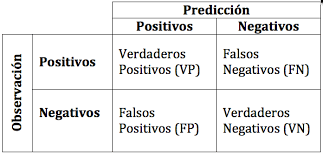
\includegraphics[width=2.5in]{images/confusion_matrix}
\end{center}
\caption{Matríz de Confusión}
\end{figure}

La estrategia solo toma la señal cuando el modelo predice un incremento en el precio, la venta por el contrario no depende del modelo, sino de los parámetros predefinidos (porcentaje de Stop Loss y Horizonte de tiempo). Esta característica implica que el valor a maximizar es la predicción de los verdaderos positivos, conocido como $Precisión$.

$$ Precisión = \frac{VP}{VP + FN} $$

\subsection{Medidas de Riesgo}

\subsubsection{Valor en Riesgo}

El valor en riesgo ó VaR por sus siglas en ingles -Value at Risk- es una medida común del riesgo implementado en instituciones financieras. Se define como la pérdida en un portafolio, tal que existe una probabilidad $p$ que las pérdidas sean iguales o mayores que el VaR y una probabilidad $(1-p)$ que sean menores que el VaR, en un tiempo determinado. Este valor se corresponde con el cuantíl de la distribución de pérdida. 

$$ Pr(Q \leq -VaR(p)) = p $$

ó

$$ p = \int_{-\infty}^{-VaR(p)}f_{q}(x)\ dx $$

siendo $f_{q}(x)$ la función de densidad de la variable aleatoria pérdida/ganancia del portafolio denotada por Q.

Aunque el VaR es utilizado comunmente en instituciones financieras e incluso exigido en alunas regulaciones como Basilea, existen varias críticas en cuanto a su implementación. Una de las críticas es su inconclusividad en cuando al tamaño de la pérdida, en este sentido, el VaR es un cuantíl de la distribución que establece un umbral en cuanto a la posible pérdida en un período, dado un nivel de significancia. Jon Danielsson (2011)

\subsubsection{Pérdida Esperada}

La pérdida esperada mejor conocida conocida como 'Expected Shortfall' -ES- es una medida alternativa al VaR que responde la pregunta ¿Cuál es la pérdida esperada cuando éstas exceden el VaR?. Formalmente la pérdida esperada se define cómo

$$ ES = E(Q/Q \leq VaR(p)) $$ 

ó utilizando la formulación matemática de esperanza

$$ ES = \int_{-\infty}^{-VaR(p)} xf_{VaR}(x)\ dx $$

Es importante acotar que para el ES existen dos fuentes de error ya que primero se debe estimar el VaR y luego obtener la esperanza de la cola de la distribución. Sin embargo es una medida que complementa el VaR. En la figura 2.2 se observa la función de densidad de una distribución normal (0,1) donde se representa el VaR y ES, el VaR vendría siendo la frontera entre las dos áreas mientras que el ES la esperanza del área azul o cola superior.
Es importante acotar que tanto el VaR como ES a pesar ser medidas de pérdidas potenciales, pueden ser referidas con signo negativo ó positivo.

\begin{figure}[H]
\setkeys{Gin}{height = .7\textwidth}
\centering
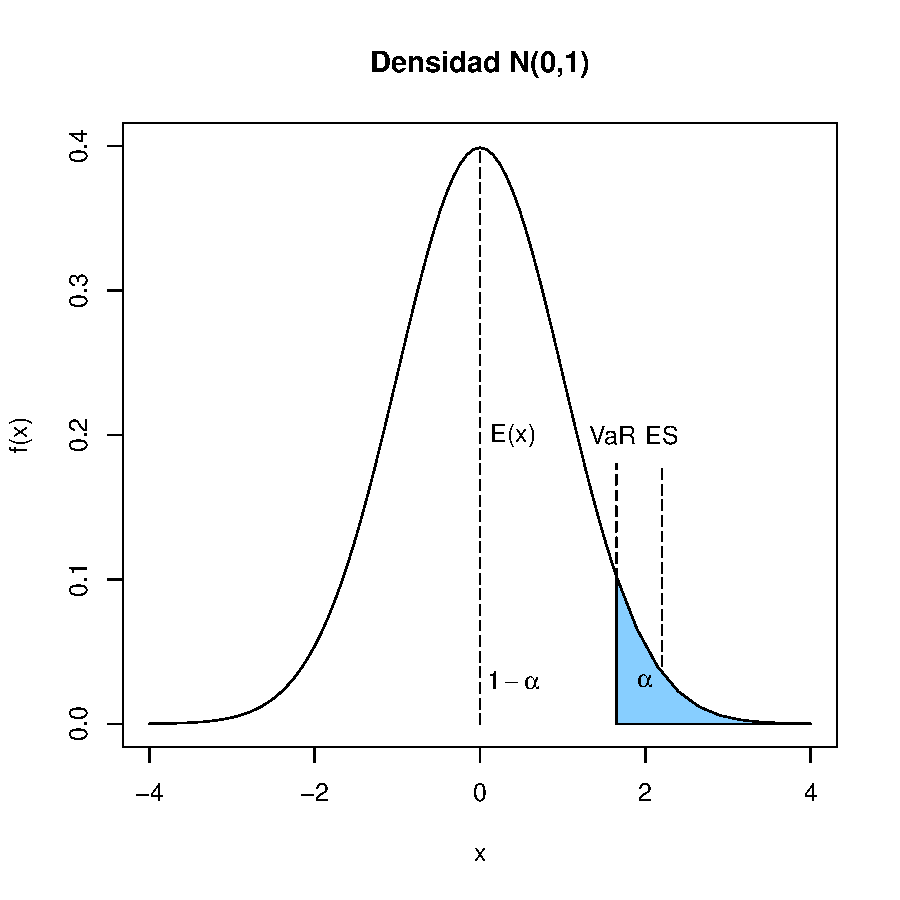
\includegraphics{main-001}
\caption{Función de densidad con VaR y ES}
\end{figure}

\section{Bases Legales}


% !TeX root = ./main.Rnw
%\SweaveUTF8

\chapter{Marco Metódico}
\section{Estrategia de Análisis}

\subsection{Datos OHLC y Fuente de los datos}

La estructura de los datos utilizados en el trabajo es de tipo OHLC por sus siglas en inglés Open, High, Low, Close. La misma, resume en 4 registros el comportamiento del precio del activo (Apertura, Cierre, Mínimo y Máximo) en un intervalo de tiempo. En el caso de la presente investigación, de un día. Este tipo de dato provee la información necesaria para cubrir las exigencia del modelo, tanto para la creación de la variable dependiente como para el cálculo de los indicadores técnicos.

Los datos fueron extraídos del portal www.investing.com, uno de los portales financieros con mayor prestigio en el mundo. Fue fundado en 2007 y es conocido por su calendario económico y directorio de brokers.

\subsection{Series de Índices Bursátiles}

El universo de estudio está representado por los índices bursátiles de los mercados financieros existentes entre el período 26/10/2008 - 18/01/2019. Un índice búrsatil es un promedio de los precios de los activos que representan un mercado o sector determinado. Los mismos sirven como 'benchmark' o referencia de la economía de un país, sector financiero, etc. En el ámbito de los 'hedge funds' son una referencia para medir la rentabilidad de una estrategia de inversión y el riesgo del mercado.

En la presente investigación se utilizan los índices como reflejo del comportamiento de varios activos, de esta manera, se mide la estrategia en un sector y no en un instrumeto en específico. Otras de las ventajas de utilizar los índices es que al representar un promedio de varios activos, sus variaciones son menos drásticas. La muestra está constituida por 5 índices bursátiles que representan distintos mercados del mundo: NASDAQ, NIKKEI, FTSE 100, BOVESPA y SP500.

\subsection{Variable Dependiente}

Las decisiones de entrada en el trading pueden ser producto de muchos factores, en la presente investigación se analiza el enfoque donde se define un porcentaje objetivo de ganancia y se intenta predecir si dicho objetivo se materializará en un futuro cercano, sin que se haya concretado una venta por Stop Loss. Este enfoque reduce la toma de decisión en una variable tal que:

$$
P_{X}(x) = 
\left\{ 
\begin{array}{ll} 
p \ ; \qquad x = c
\\
\\
1-p \ ; \qquad x = -d
\end{array}
\right
$$

Dado los datos OHLC del activo es posible identificar los períodos en donde se materializa la variable dependiente. la identificación se realiza, comparando el precio de cierre con los precios máximos y mínimos de las siguientes h observaciones, donde h es el número de períodos, en este caso días en los cuales se desea evaluar la condición.

En la práctica se identifica los registros que cumplen con esta condición añadiendo una columna a la data donde incluimos 'buy' para identificar los registros donde se da la señal y 'stay' en caso de que no haya ocurrido o hubiese ocurrido primero el retroceso del precio.

\subsection{Variables Predictoras}

Los indicadores a utilizar fueron seleccionados buscando recoger la mayor información posible sobre el precio del activo, se pueden resumir en tres categorías: tendencia, momentum y volatilidad.

No es de interés en la presente investigación describir como funciona cada indicador para la toma de decisiones en el trading basado en fundamentos técnicos. Cada indicador puede utilizarse de distintas maneras, calcularse con distintos parámetros y asociarse a discreción del trader, lo que conlleva a un sin fin de reglas de asciación. 

Lo que busca la investigación es utilizar la relación entre los indicadores como variables independientes que ayuden al modelo a predecir oportunidades de entradas. En este sentido se asume la existencia de una dinámica local del mercado que puede ser predecida con ayuda de estos indicadores. Algunos de los indicadores inicialmente escogidos para el modelo fueron excluidos debido a la alta correlación que presentaban. A continuación se presentan los indicadores utilizados:

\begin{itemize}
\item Retornos con respecto al precio de Cierre.
\item RSI (Relative Strength Index) de 14 períodos, el cual es un indicador de volatilidad.
\item MACD (Moving Average Converge/Divergence) el cual es una diferencia de dos EMAs (Exponential Moving Average) de 12 y 26 períodos. Este es un indicador de tendencia que se complementa con un EMA de 9 períodos. 
\item ADX (Average Directional Index), este es un indicador que utiliza dos indicadores de dirección +Di y -Di, se calculó en base a 14 períodos y mide tendencia.
\item Bandas de Bollinger, el cual es un indicador de tendencia y volatilidad, utiliza dos bandas calculadas a partir de una media movil con desviaciones estándar. Se utilizó en base a 14 períodos y una desviación de 2.5.
\item ATR (Average True Range), es un indicador de volatilidad calculado a partir de los máximos y mínimos de un período, en este caso 14.
\end{itemize}

Estos indicadores están fuertemente correlacionados por lo que se decidió, disminuir el número de variables dejando solo las más representativas de cada indicador.

Ahora bien, la idea base de la investigación era utilizar los valores de cada indicador como variables predictora. Dado que el cálculo de todos los indicadores provienen de la misma variable -precio del activo, en la mayoría de los casos precio de cierre-, exite una alta colinealidad entre ellos, la idea de utilizar el ACP es precisamente para enfrentar este problema como se detallará más adelante. Sin embargo, es de notar que los valores de los indicadores por sí solos no proveen un poder predictivo, lo que realmente usa el trader son las asociaciones entre indicadores para encontrar patrones. 

Se decidió entonces, utilizar como predictores no los indicadores por si solos, sino, las relaciones entre cada uno de ellos. Esto se abordo agregando al modelo las interacciones entre todos los indicador, y removiendo los valores de los indicadores por sí solos. De esta manera el hecho de utilizar ACP, no solo es visto ahora como una manera de remover la colinealidad entre predictores sino como método de reducción de variables, ya que el modelo pasó de tener 10 predictores -incluyendo el precio de cierre- a 45.

\subsection{Validación Cruzada en Series de Tiempo}

La validación Cruzada es un metódo de validación y prueba que consiste en dividir los registros aleatoriamente en grupos de similar tamaño. El primer grupo es utilizado como validación del modelo que ha sido entrenado en el resto de los datos, este proceso se realiza k veces, y el resultado final es el promedio arrojado por cada una de las k validaciones.

Ahora bien este método asume que no existe relación entre las observaciones, es decir que son independientes. Esto no es verdad en el caso de las series de tiempo debido a la condicion de autoregresión. Por lo tanto al dividir la data se debe respetar el orden temporal de cada observación. 

\subsection{WalkForward Backtesting}

Al principio de la investigación se implementó el método de entrenamiento, validación y prueba comúnmente utilizado, en donde la mayor parte de la data es destinada a entrenamiento del modelo, otra seccion es destinada a validación, para elegir los parámetros óptimos, y finalmente se testeaba el modelo en la data de prueba. Sin embargo este tipo de metodología en opinión del investigador no es el más óptimo para desarrollar el presente modelo, dado el dinamísmo de los mercados bursátiles la estrategia no puede permanecer estática en el tiempo.

Para contrarestar esta situación se opto por el método de $backtesting Walkforward$, el cual consiste en entrenar el modelo en un período base de data, en este caso los primeros 4 años de estudio, posteriormente se aplica la estrategia en el año siguiente y se obtiene los primeros resultados. Luego este año de aplicación es incluído en la data de entrenamiento -es decir, la data de entrenamiento pasa a ser de 5 años- y se evalúa el modelo en el siguiente año. De esta manera, contemplamos el dinamísmo del mercado permitiendole al modelo -y por ende a la estrategia- utilizar el período mas reciente con respecto al cual será implementado. En la presente figura se ilustra la metodología implementada.

\begin{figure}[ht]
\begin{center}
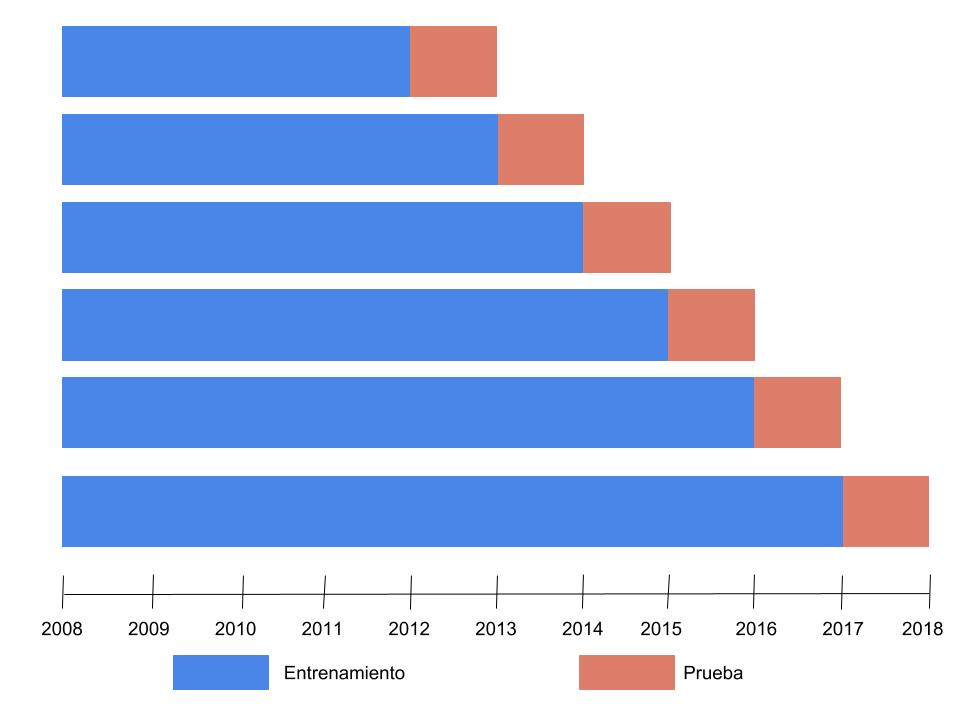
\includegraphics[width=2.5in]{images/walkforward_plot}
\end{center}
\caption{Metodología WalkForward}
\end{figure}

Otra de las caracteristicas de la metodología que se modificó fue la elección de los parámetros óptimos. Previamente se utilizaba la data de validación para buscar la combinación de parámetros óptima. Ahora bien en la metodología de Walkforward se utilizan los mismo parámetros. A opinión del investigador al buscar los mejores parámetros se estaría incurriendo en un posible cesgo de sobreoptimización. El hecho de que en un año determinado unas configuraciones óptimas den los mejores resultados no asegura que se replique en el siguiente año.

La selección de los parámetros debería ser un estudio previo de la serie financiera a testear. Evidentemente al seleccionar un período de tiempo mas corto se obtendrán menos observaciones que cumplan con el patrón por lo tanto se estaría en presencia de un problema de data imbalanceada que debe tener un tratamiento distinto. Por otro lado el utilizar un horizonte mayor no representa gran cambio en el número de ocurrencias, pero sí en el caso de que la transacción quede abierta -hay recordar que h representa una condición de salida para la estrategia de no ocurrir el target ni el stop loss-. La estrategia implementada en la invstigación toma un horizonte de 20 períodos ya que este valor representa un umbral para la ocurrencia del objetivo.


\begin{figure}[H]
\setkeys{Gin}{width = 0.8\textwidth}
\centering
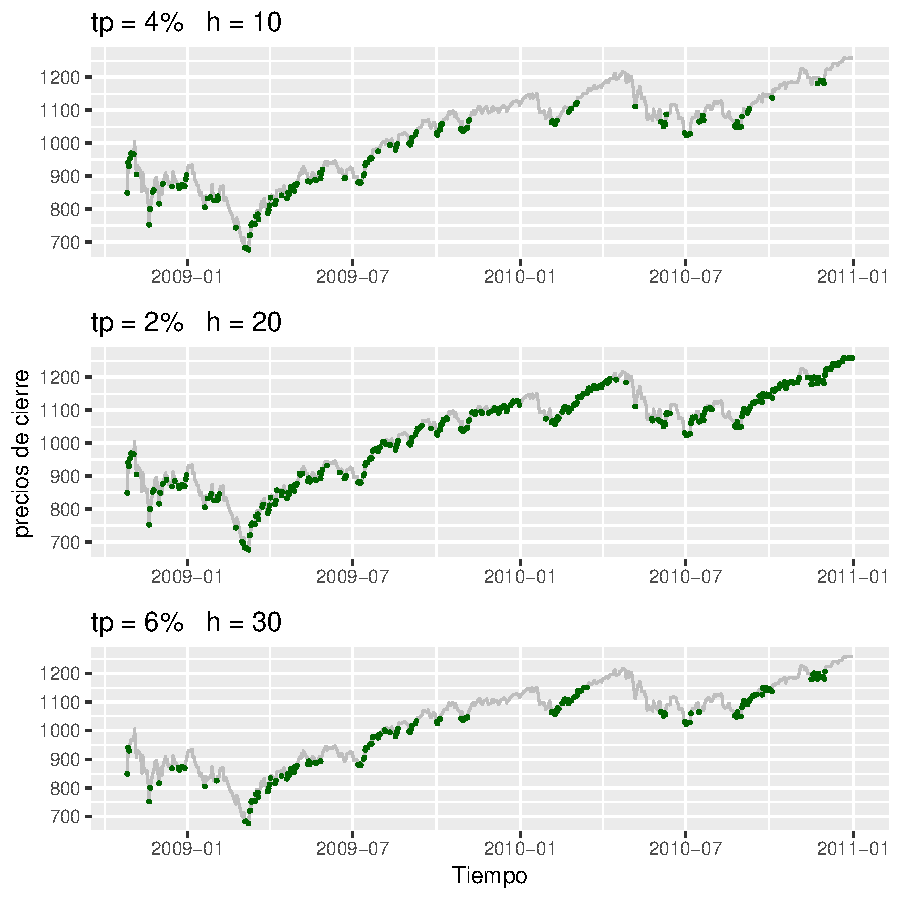
\includegraphics{main-003}
\caption{Observaciones que presentan ocurrencias con sl = 2.5\%, en el primer conjunto de datos de entrenamiento (26/10/2008 - 31/12/2010) para el índice S\&P500, para diferentes valores de tp y h}
\end{figure}


\subsection{Reducción de la dimensión con ACP}

La técnica que utiliza el ánalisis de componentes principales (PCA) para reducir el número de variables predictoras es conocido como Principal Component Regression (PCR). PCR es utilizado para extraer la información más importante de una matríz de datos multivariante y expresar ésta información en nuevas variables llamadas componentes principales. Éstas son una combinación lineal de las variables originales. Aunque el número de componentes principañes puede ser igual al número de variables, la idea es utilizar un grupo reducido de componentes que maximizen la variación.

Por su parte el modelo propuesto utiliza las interacciones entre las variables predictoras, esto aumenta el número de variables de 10 a 45, las cuales además en muchos casos están correlacionadas. Al utilizar PCR se reduce el número de variables en la mayoría de los casos a 7 componentes donde las dos primeras contienen al rededor del 25\% de la variación, es importante recordar que esta reducción se realiza en cada período de entrenamiento. Para el modelo se estableció que en cada período de entrenamiento se utilizaría la cantidad de componentes necesarias para explicar el 85\% de la variación de la matríz de datos.

\subsection{Modelado de los Retornos}

Tal como se establece en la sección -- la variable aleatoria retorno del trade puede obtener 2 posibles valores, si el trade es exitoso toma el valor c con probabilidad p, en caso contrario toma el valor -d con probabilidad 1-p. Para cada activo se puede asumir p como la probabilidad positiva -precisión- obtenida en el modelo. Por su parte c y -d son fijados en 20 y -25 respectivamente, esto viene dado por haber establecido los porcentajes de salida en 0.02 de ganancia y 0.025 de perdida y asumir un capital a riesgo en cada trade de 1000 unidades.

Asumiendo que la ocurrencia de los trades se distribuye de manera uniforme en el tiempo, y con un número de muestra suficientemente grande podemos concluir que

$$ \frac{\sum x_{i} + nE(x)}{n\sigma_{x}} \sim N(0,1) $$

siendo

$$ E(x) = pc - (1-p)d \qquad y \qquad \sigma_{x} = (pc - (1-p)d)^{2} - (pc^{2} - (1-p)d^{2}) $$

Es posible modelar los retornos producidos por la estrategia y calcular el valor a riesgo -VaR- y pérdida esperada -ES- dado un número de operaciones. Tanto el VaR como el ES son medidas comunmente utilizadas para representar el riesgo de pérdida en un período de tiempo determinado, en este caso, se establecerá en vez de tiempo, un número de trades cerrados por la estrategia.

Dado que el retorno de la estrategia se distribuye N(0, 1), se definen el VaR y ES cómo

$$ VaR_{\alpha} = \sigma \Phi^{-1}(\alpha) + \mu $$

$$ ES_{\alpha} = \sigma \frac{\phi(\Phi^{-1}(\alpha))}{1-\alpha} + \mu $$

En la presente investigación se establecen $n = 200$ y $\sigma = 0.95$. Es decir que el VaR puede interpretarse como: "Existe una probabilidad del 5\% que la estrategia genere una pérdida igual ó menor que $VaR_{\alpha}$, luego de 200 trades realizados".

Mientras que el ES se interpreta como: "En caso de que la estrategia genere una pérdida mayor que $VaR_{\alpha}$ luego de 200 trades, se espera que ésta pérdida sea de $ES_{\alpha}$"
% !TeX root = ./main.Rnw
%\SweaveUTF8

\chapter{Análisis de Resultados}

\section{Análisis Exploratorio de los datos}

\subsection{Análisis de los Índices}

En la figura -- se observa el precio de cierre de cada índice durante el período de estudio. Se puede apreciar que en general los cinco mercados tienen tendencia a la alta. En general para el S\&P y NASDAQ se aprecia una menor variabilidad que en los demás índices.

Las curvas del S\&P y NASDAQ son muy parecidas ya que ambas representan cotizaciones de las mayores empresas americanas. Se aprecia un crecimiento sostenido desde el año 2009, con algunos períodos mas estables, a principios del 2016 -por la polémica victoria de Donald Trump como presidente- y en 2018 provocado por el miedo a un incremento en las tasas de interés por parte de la Reserva Federal y las tensas negociaciones con China.

Por su parte el NIKKEI es el índice búrsatil de la bolsa de Tokio, resume las cotizaciones de 225 grandes empresas de Japón de distintos sectores industriales. Al ver la gráfica de sus cotizaciones se observa un rápido crecimiento entre 2009 y 2010, sin embargo con la ocurrencia del terremoto registrado en el norte del país a principios del 2011 el índice se vio afectado y llegó a su nivel más bajo de 8160 puntos el 25 de noviembre desde el 10 de marzo de 2009. La recuperación ocurrió en 2013 debido a los cambios implementados por el país en materia de política fiscal y monetaria. El Gobierno impulsó el gasto público y el Banco Central de Japón inyecto dinero en la economía a gran escala.

El FTSE 100 es un índice búrsatil calculado con las cotizaciones de las 100 empresas más grandes de Reino Unido, en su gráfica se observa una tendencia alcista aunque con mayor ruido o variabilidad que los otros indices. Se puede apreciar una caída en las cotizaciones el año 2015 debido a resultados negativos mostrados por la actividad manufacturera en Asia, especialmente en China. Esto afecta los mercados europeos dada que este es el principal consumidor del mercado asiático.

Por último el índice BOVESPA representa las 50 empresas de mayor capitalización de la Bolsa de Valores de Sao Paulo. Se aprecia que a diferencia de los anteriores, éste mantiene una tendencia a la baja hasta 2016 debido a la recesión económica sufrida por Brasil mostrando una contracción del PIB en un 3.8\% para 2015. Aunado a factores ambientales como el virus del Zika y el ecándalo de corrupción de Petrobras. A partir de 2016 con la inflación gradualmente bajo control y tasas de interés en decrecimiento, la confianza de los inversores llevó a un rapido crecimiento del índice en los últimos tres años.


\begin{figure}[H]
\setkeys{Gin}{width =0.8\textwidth}
\centering
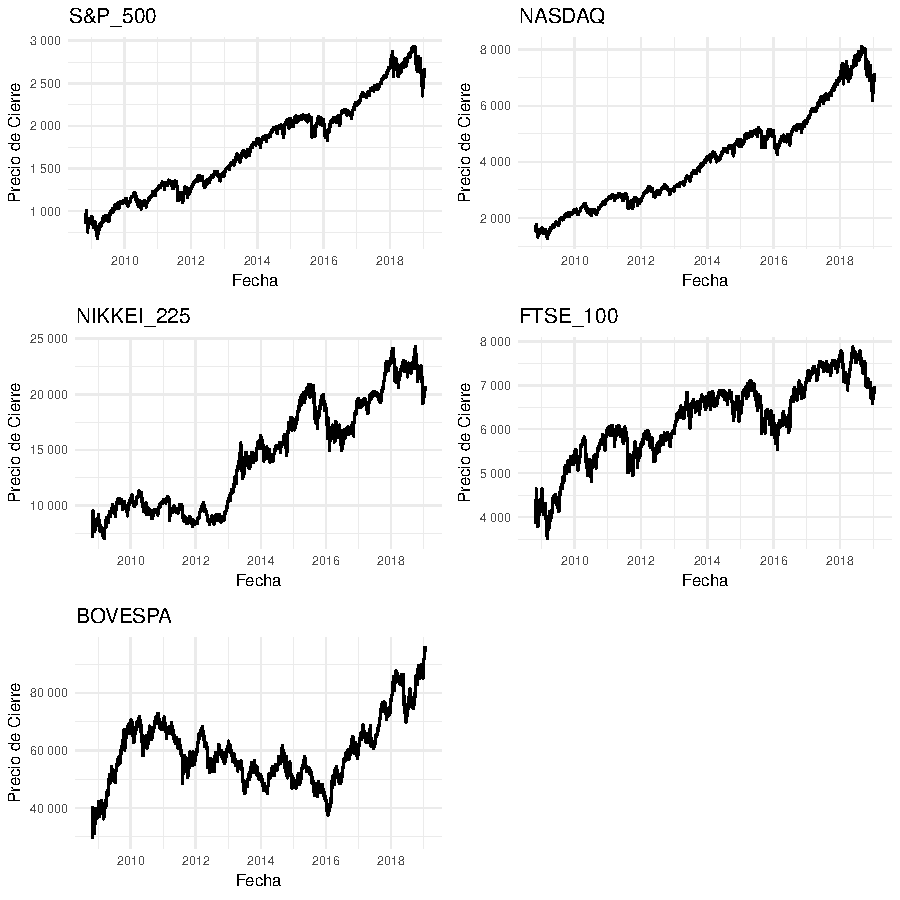
\includegraphics{main-005}
\caption{Precios de Cierre de los índices en el período de estudio (26/10/2008 - 18/01/2019)}
\end{figure}


\subsection{Análisis de las Variables Predictoras}

En la figura -- se observa la correlación de las variables originales para el primer período de entrenamiento del índice S\&P500. Como se puede observar existe alta correlación entre las distintas variables del precio (Apertura, Cierre, Máximo y Mínimo) por lo que se decidió trabajar solo con los precios de cierre dado que ésta es la misma utilizada para determinar la variable dependiente. Así mismo se observa alta correlación entre los rezagos de los rendimientos, para esto se decidió trabajar solo con los rezagos de 1, 3 y 5 períodos. Por su parte se descarta la variable dip -elemento utilizado en el indicador ADX- por su fuerte correlación con el RSI. Se determina lo mismo para la banda inferior del indicador de Bollinger. En la figura -- se muestra las correlaciones de las variables definitivas

\begin{figure}[H]
\setkeys{Gin}{width = 0.6\textwidth}
\centering
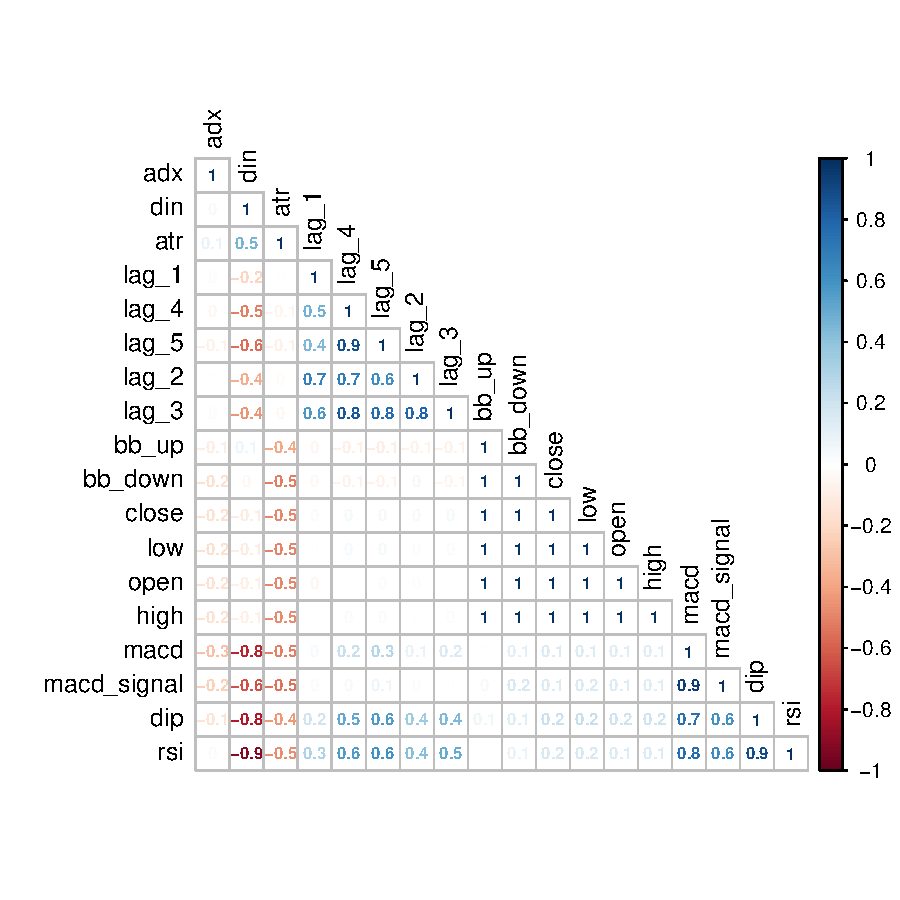
\includegraphics{main-006}
\caption{Correlación entre indicadores originales calculados con los precios del S\&P500 en el primer período de entrenamiento(01/01/2009 - 31/12/2012)}
\end{figure}


\begin{figure}[H]
\setkeys{Gin}{width = 0.6\textwidth}
\centering
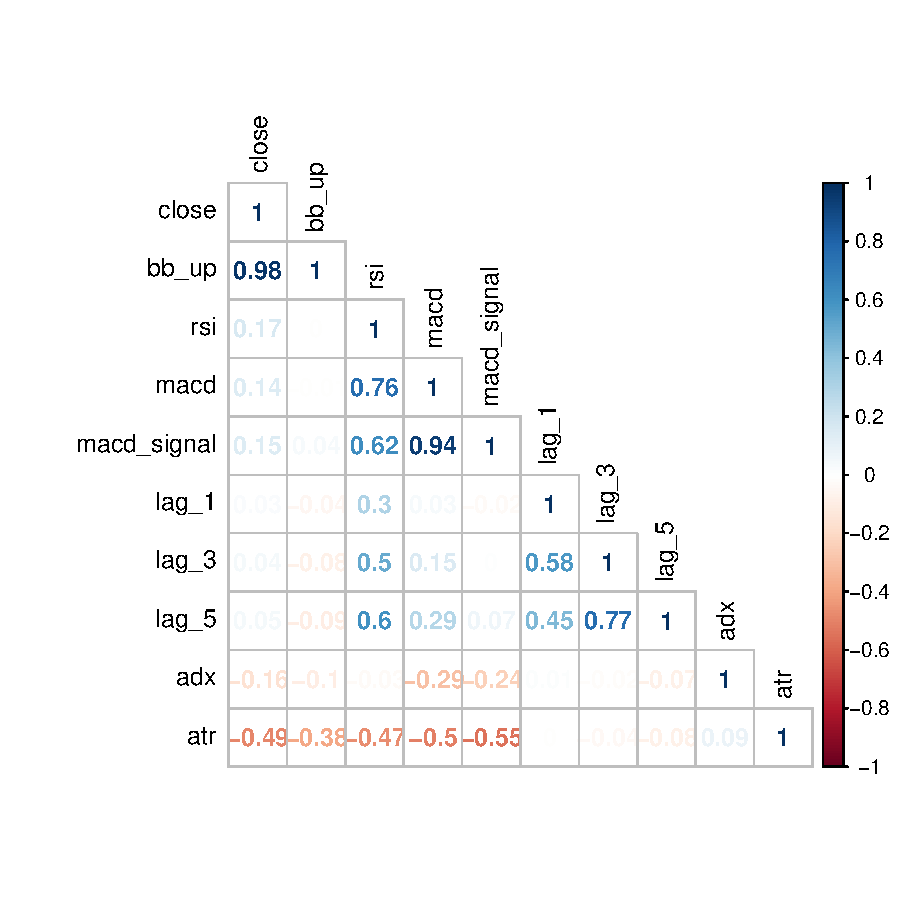
\includegraphics{main-007}
\caption{Correlación entre indicadores definitivos calculados con los precios del S\&P500 en el primer período de entrenamiento(01/01/2009 - 31/12/2012)}
\end{figure}

A continuación se presentan una serie de gráficos para reflejar lo anteriormente expuesto en cuanto a la relación entre los indicadores.


\begin{figure}[H]
\centering
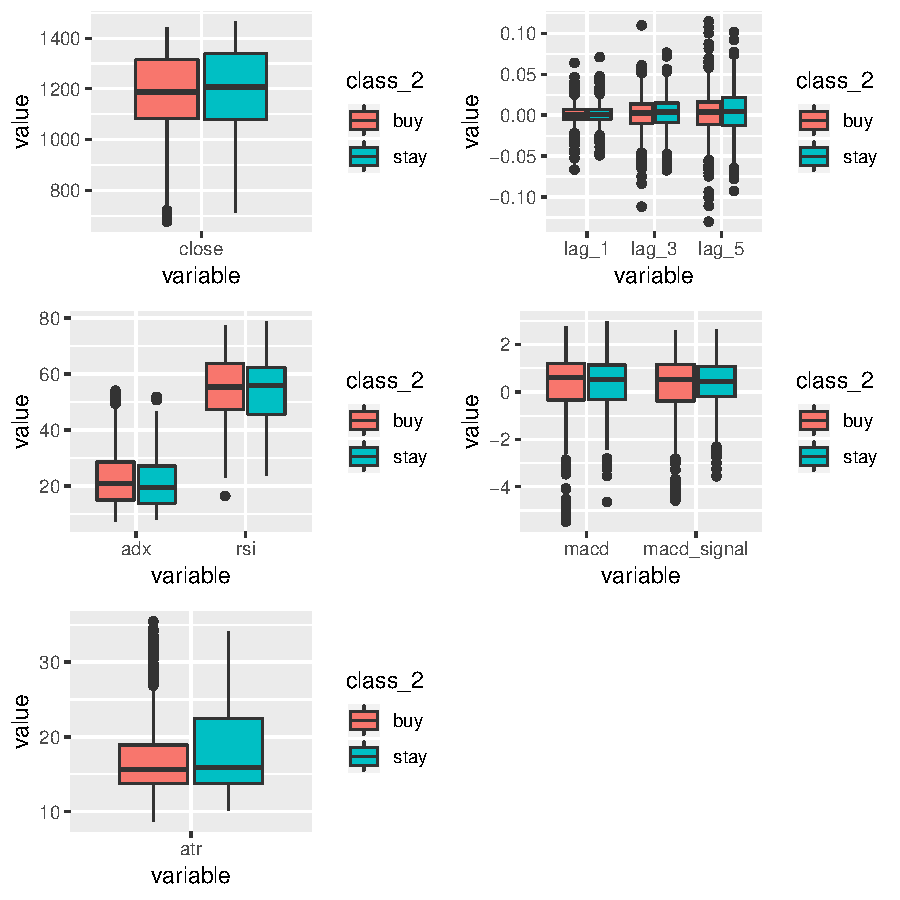
\includegraphics{main-009}
\caption{Gráfico de cajas de indicadores definitivos calculados con los precios del S\&P500 en el primer período de entrenamiento(01/01/2009 - 31/12/2012)}
\end{figure}

\begin{figure}[H]
\centering
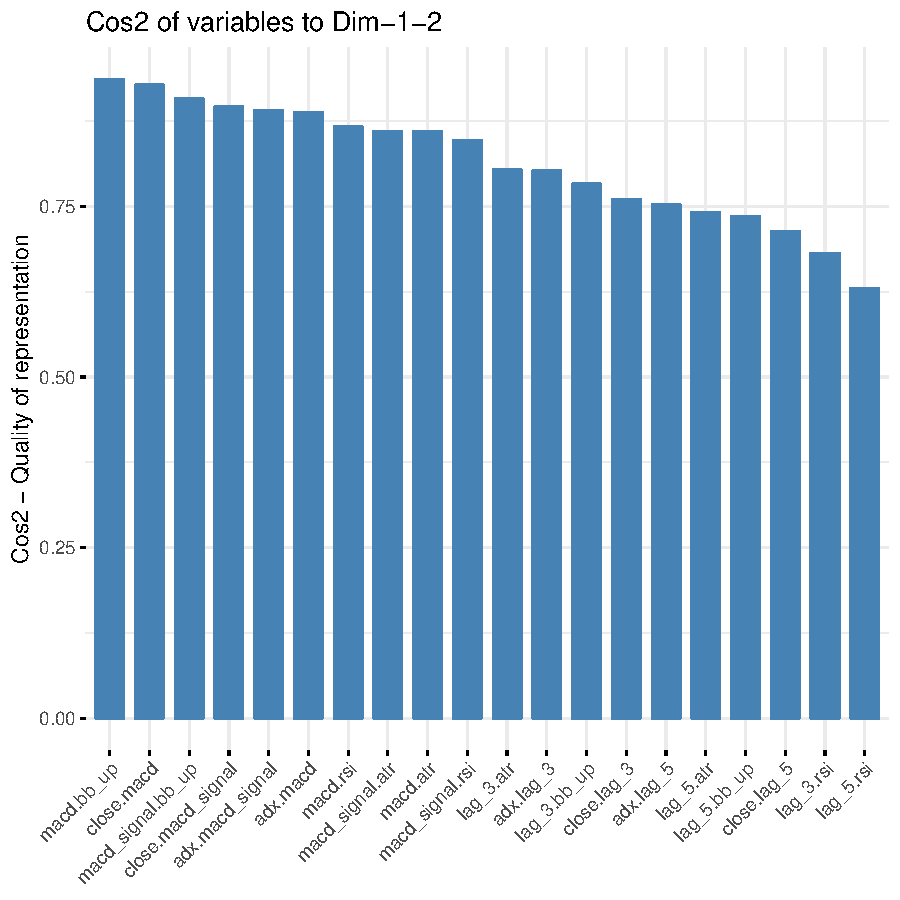
\includegraphics{main-010}
\caption{Histogramas de frecuencia de indicadores definitivos calculados con los precios del S\&P500 en el primer período de entrenamiento(01/01/2009 - 31/12/2012)}
\end{figure}

\begin{figure}[H]
\centering
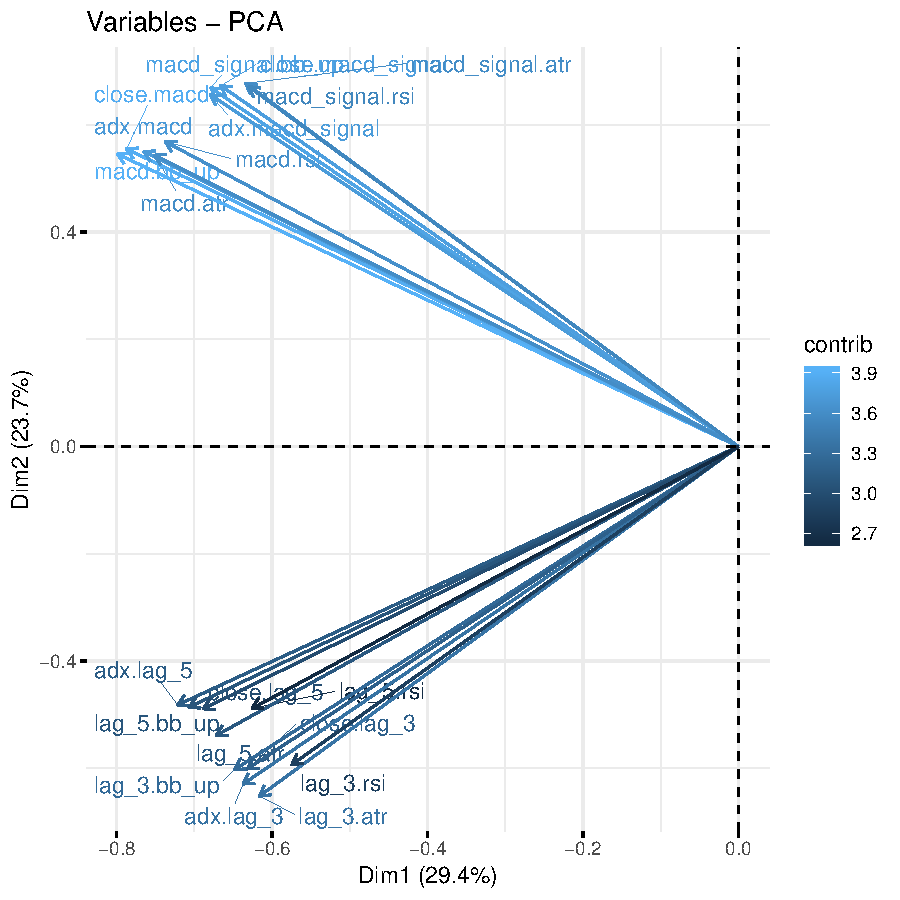
\includegraphics{main-011}
\caption{Gráfico de densidad de indicadores definitivos calculados con los precios del S\&P500 en el primer período de entrenamiento(01/01/2009 - 31/12/2012)}
\end{figure}

\subsection{Resultados del ACP}

A continuación se analizan los resultados de los componentes arrojados por el modelo en el primer período de entrenamiento (2009-2012) utilizando el índice S\&P500, en esta sección se referira a ésta como 'matriz de datos'. Ahora bien, si se quisiera analizar cada una de las componentes arrojadas en cada muestra de entrenamiento se necesitaría repetir este análisis 30 veces lo cual no es práctico para los fines de la investigación. En este sentido se elaboró una aplicación con el paquete Shiny de R, para visualizar de manera interactiva las gráficas que ayudan a entender los componentes. La aplicación puede ser visitada con el siguiente enlace https://rodserr.shinyapps.io/trading-ML/.


Los eigenvalores miden la cantidad de variación retenida por cada componente. Los eigenvalores son mayores para los primeros componentes, dado que el primer componente busca maximizar la cantidad de variación de la matriz de datos, por lo que cada vez es menor la cantidad de variación retenida por cada componente.

La proporción de variación explicada por cada eigenvalor viene dada de dividir cada eigenvalor por su sumatoria, en este caso 45 -el número de variables originales-.

Un eigenvalor mayor que 1 indica que el componente tiene mayor variación que la contenida en una de las variables originales. En la figura -- Se puede observar que el 85\% de la variación esta contenida en los primeros 7 componentes. Igualmente se aprecia que el eigenvalor de los 10 PCs es mayor que 1. 

\begin{figure}[H]
\setkeys{Gin}{width = 0.8\textwidth}
\centering
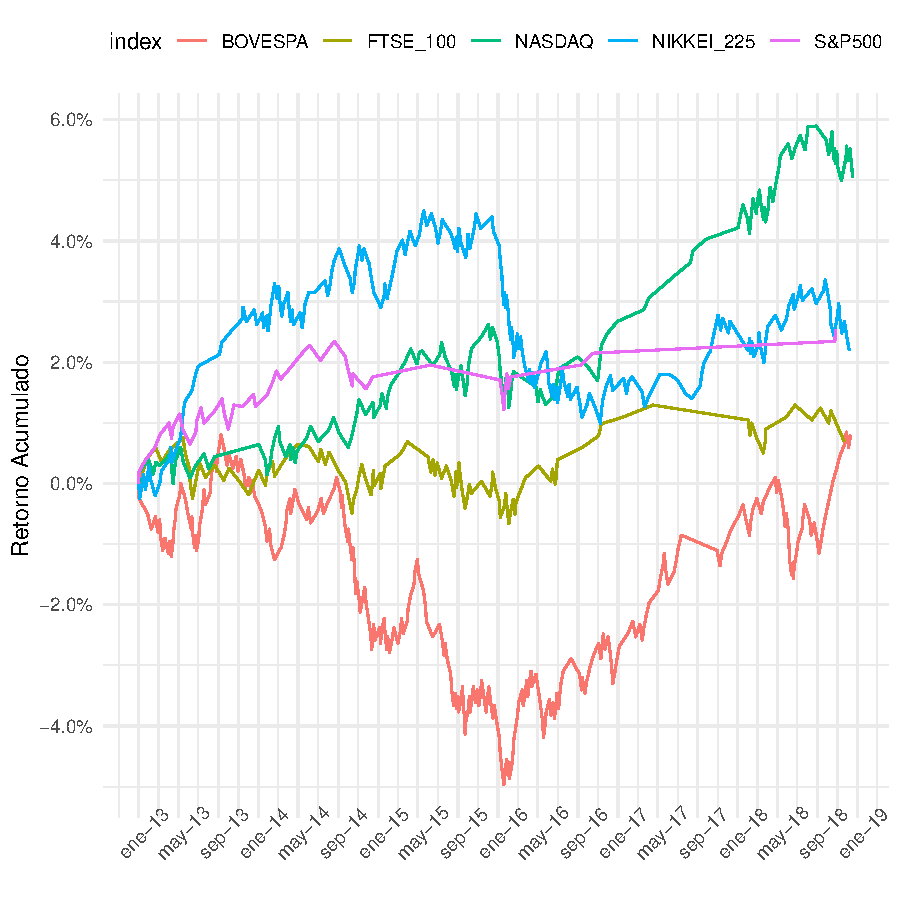
\includegraphics{main-013}
\caption{Eigenvalores y Porcentaje de contribución para los 10 componentes más importantes obtenidos por la matríz de datos}
\end{figure}

La contribución de las variables representan la variabilidad contenida en un componente. Las variables correlacionadas con el componente principal 1 (PC1) y PC2 son las más importantes en explicar la variabilidad en la matráz de datos. Aquellas que no se correlacionan con ninguna componente son desechadas por su baja contribución. En la figura -- se observa la contribución de las primeras 30 variables en PC1, PC2 y la contribución obtenida en ambas.

\begin{figure}[H]
\setkeys{Gin}{width = 0.8\textwidth}
\centering
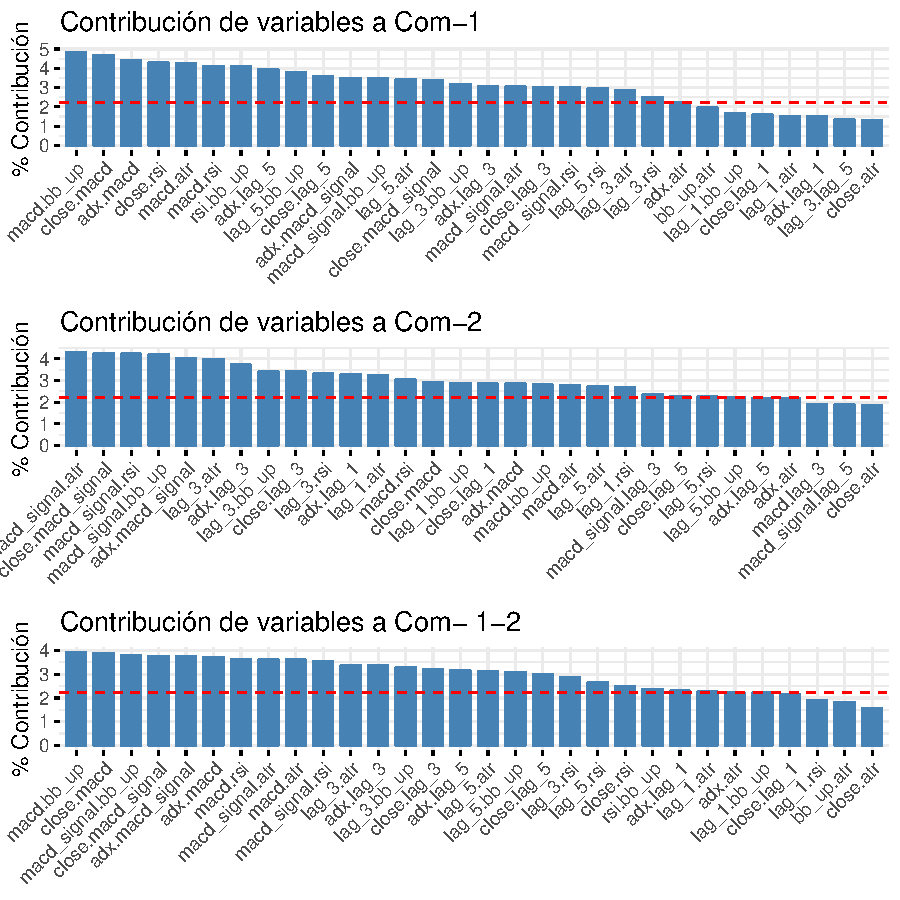
\includegraphics{main-014}
\caption{Contribución de cada variable para PC1, PC2 y el total de la contribución en ambos componentes}
\end{figure}

La línea roja indica el promedio esperado de contribución si las variables fueran uniformes, es decir $ \frac{1}{N° de Variables} = \frac{1}{45} = 2,2\%$. Una variable sobre este umbral se considera importante en la contribución al componente. Se aprecia como las interacciones que predominan en ambos componentes estan relacionadas con el indicador MACD.

La calidad de representación en el gráfico viene dada por el valor de $Cos^2$, el cual se refiere a la importancia que tiene la variable para interpretar el componente. Para una variable la suma de $Cos^2$ en todas las componentes equivale a 1. En la figura -- se muestra los valores de $Cos^2$ para las primeras 2 componentes

\begin{figure}[H]
\setkeys{Gin}{width = 0.8\textwidth}
\centering
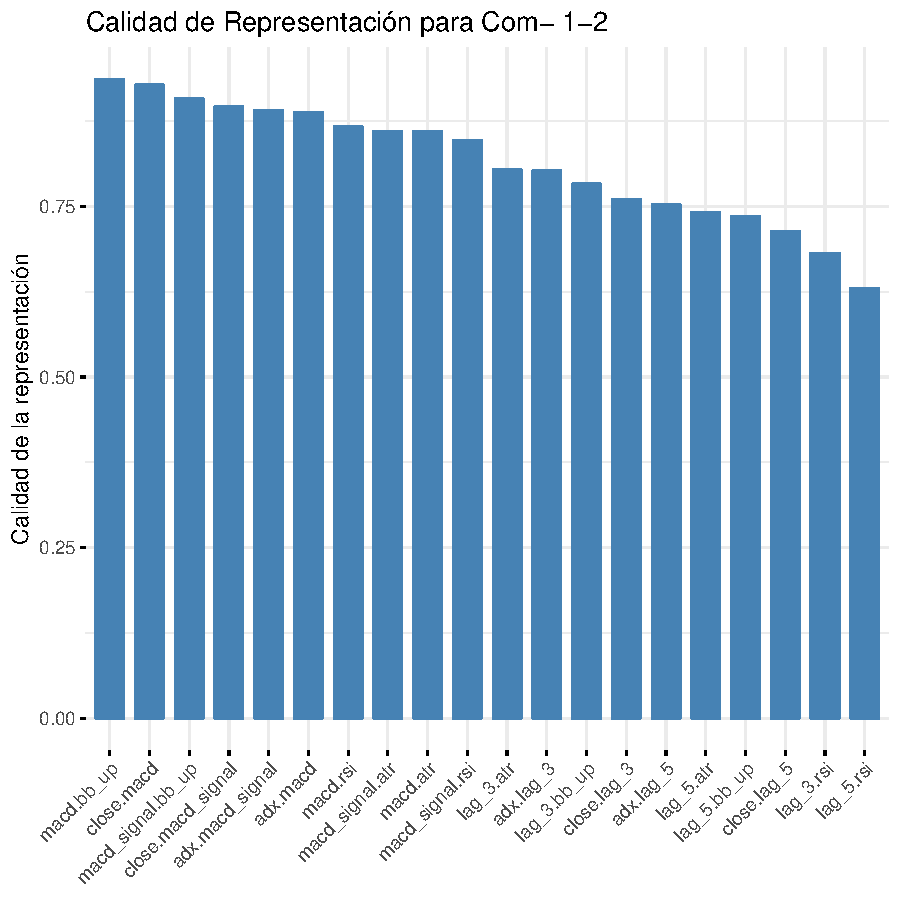
\includegraphics{main-015}
\caption{Calidad de representación medida por $Cos^2$ de cada variable en PC1 y PC2}
\end{figure}

El gráfico de correlación ó Factor map muestra la relación entre las variables. Las claves para su interpretación son:

\begin{itemize}
\item Las variables positivamente correlacionadas se encuentran agrupadas entre sí
\item Las variables negativamente correlacionadas se posicionan en quadrantes opuestos.
\item La distancia entre las variables y el origen mide la calidad de representación de las variables en el gráfico. Mientras más alejado del origen, mejor representadas 
\end{itemize}

En la figura -- se observa el gráfico de correlación para PC1 y PC2, el color de cada variable viene dado por su contribución, mientras más oscuro menor es su contribución a los componentes. Se puede apreciar que las variables con mayor contribución están agrupadas por dos tipos de indicadores predominantes, en el cuadrante superior izquierdo aparecen variables constituidas por interacciones con los indicadores del MACD, mientras que en el cuadrante inferior izquierdo los indicadores predominantes son los rezagos. Por otro lado los grupos forman un ángulo de 90° por lo que no están correlacionados.

\begin{figure}[H]
\setkeys{Gin}{width = 0.8\textwidth}
\centering
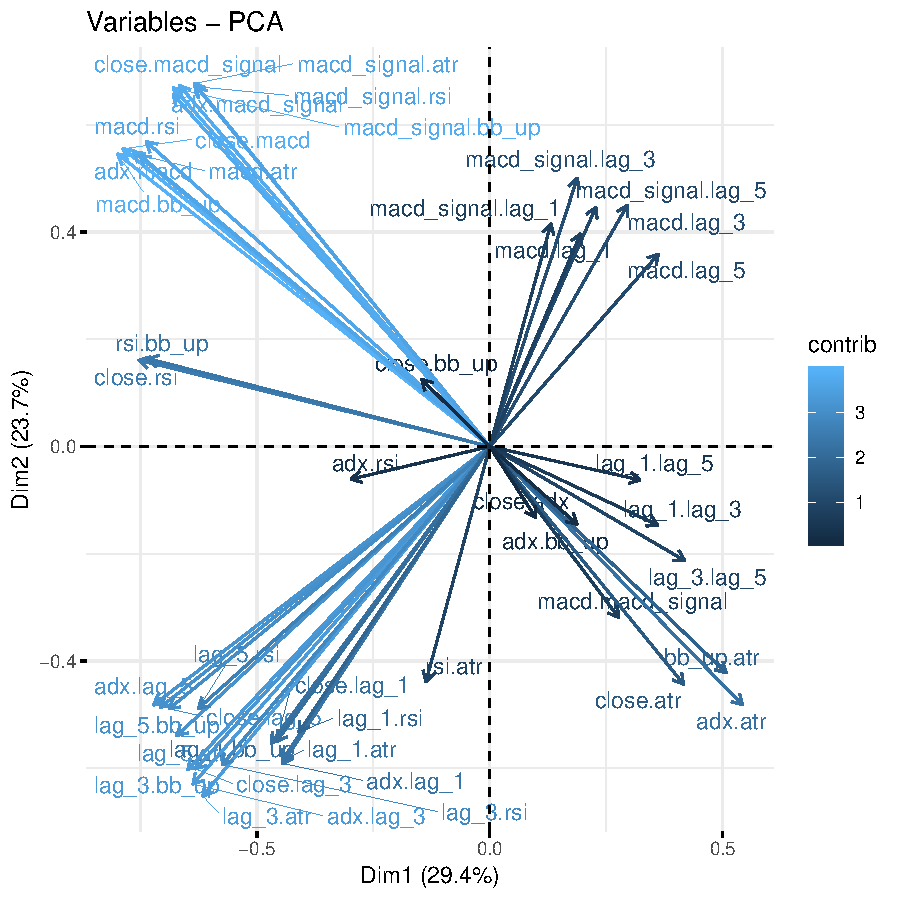
\includegraphics{main-016}
\caption{Gráfico de Correlación entre PC1 y PC2}
\end{figure}

En la figura -- se muestran los gráficos de dispersión entre los componentes, 


\begin{figure}[H]
\setkeys{Gin}{width = 1\textwidth, height = 1.2\textwidth}
\centering
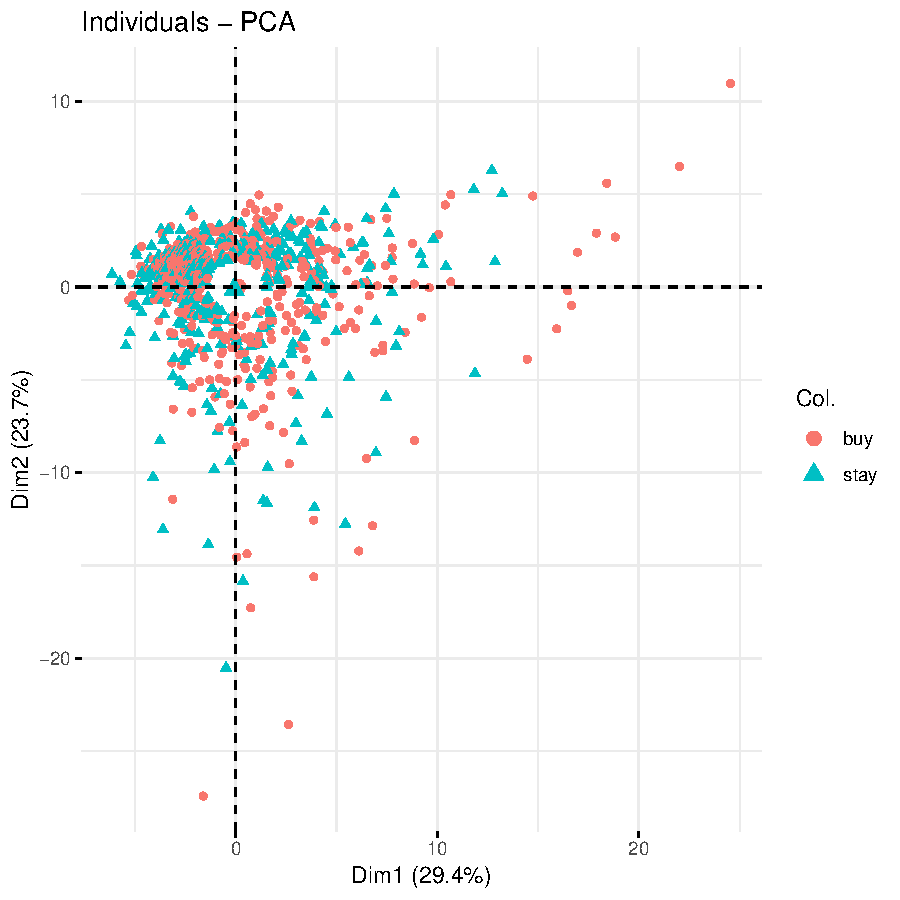
\includegraphics{main-018}
\caption{Gráfico Dispersión entre los componentes. Los puntos rojos representan las observaciones marcadas como 'buys', los triángulos azules los 'stays'}
\end{figure}

%%%%%%%%%%%%%%%%%%%%%%%%%%%%%%%%%%%%%%%%%%%%%%%%%%%%%%%%%%%
%%%%%%%%%%%%%%%%%%%%%%%%%%%%%%%%%%%%%%%%%%%%%%%%%%%%%%%%%%%
%%%%%%%%%%%%%%%%%%%%%%%%%%%%%%%%%%%%%%%%%%%%%%%%%%%%%%%%%%%
%%%%%%%%%%%%%%%%%%%%%%%%%%%%%%%%%%%%%%%%%%%%%%%%%%%%%%%%%%%
%%%%%%%%%%%%%%%%%%%%%%%%%%%%%%%%%%%%%%%%%%%%%%%%%%%%%%%%%%%
%%%%%%%%%%%%%%%%%%%%%%%%%%%%%%%%%%%%%%%%%%%%%%%%%%%%%%%%%%%
%%%%%%%%%%%%%%%%%%%%%%%%%%%%%%%%%%%%%%%%%%%%%%%%%%%%%%%%%%%
%%%%%%%%%%%%%%%%%%%%%%%%%%%%%%%%%%%%%%%%%%%%%%%%%%%%%%%%%%%
%%%%%%%%%%%%%%%%%%%%%%%%%%%%%%%%%%%%%%%%%%%%%%%%%%%%%%%%%%%
%%%%%%%%%%%%%%%%%%%%%%%%%%%%%%%%%%%%%%%%%%%%%%%%%%%%%%%%%%%


\newpage

\section{Coeficientes del modelo}

En el presente capítulo se realiza la descripción de los resultados obtenidos despues de la aplicación del método propuesto para la estrategia. De igual modo, se presentan los resultados arrojados por las pruebas de Backtesting simulando las entradas y salidas. Los nombres de los componentes fueron sustituidos por etiquetas que intentan explicar la representación del componente en el modelo con ayuda de las gráficas mostradas en la sección 4.1.3


En la tabla 4.1 se describen los resultados de los parámetros arrojados por la regresión logística en los 6 períodos de entrenamiento para la serie del S\&P500.

\begin{center}
\captionof{table}{Resumen del modelo para cada período de entrenamiento utilizando S\&P500}
\captionof*{table}{Período de entrenamiento 2009 - 2012}
% latex table generated in R 3.5.3 by xtable 1.8-3 package
% Thu Mar 14 23:34:00 2019
\begin{table}[ht]
\centering
\begin{tabular}{rrrrr}
  \hline
 & Estimate & Std. Error & z value & Pr($>$$|$z$|$) \\ 
  \hline
(Intercept) & -0.36 & 0.06 & -5.58 & 0.00 \\ 
  ATR.Pos-Macd.Neg & -0.01 & 0.02 & -0.81 & 0.42 \\ 
  Macd.Pos-Rezago.Neg & -0.01 & 0.02 & -0.66 & 0.51 \\ 
  ADX.Pos-Macd.Neg & 0.01 & 0.03 & 0.15 & 0.88 \\ 
  Rezago.Pos-ADX.Neg & 0.09 & 0.04 & 2.47 & 0.01 \\ 
  Bollinger.Pos-Rezago.Neg & -0.02 & 0.04 & -0.60 & 0.55 \\ 
  Macd.Pos-RSI.Neg & -0.02 & 0.04 & -0.37 & 0.71 \\ 
  ATR.Pos-RSI.Neg & 0.11 & 0.05 & 2.18 & 0.03 \\ 
   \hline
\end{tabular}
\end{table}\end{center}

\begin{center}
\captionof*{table}{Período de entrenamiento 2009 - 2013}
% latex table generated in R 3.5.3 by xtable 1.8-3 package
% Thu Mar 14 23:34:00 2019
\begin{table}[ht]
\centering
\begin{tabular}{rrrrr}
  \hline
 & Estimate & Std. Error & z value & Pr($>$$|$z$|$) \\ 
  \hline
(Intercept) & -0.41 & 0.06 & -7.06 & 0.00 \\ 
  ATR.Pos-Macd.Neg & 0.02 & 0.02 & 1.35 & 0.18 \\ 
  Macd.Pos-Rezago.Neg & -0.01 & 0.02 & -0.40 & 0.69 \\ 
  ADX.Pos-Macd.Neg & 0.02 & 0.03 & 0.58 & 0.56 \\ 
  Rezago.Pos-ADX.Neg & 0.05 & 0.03 & 1.75 & 0.08 \\ 
  Bollinger.Pos-Rezago.Neg & 0.02 & 0.03 & 0.71 & 0.48 \\ 
  Macd.Pos-RSI.Neg & 0.04 & 0.04 & 1.08 & 0.28 \\ 
  ATR.Pos-RSI.Neg & -0.12 & 0.04 & -2.95 & 0.00 \\ 
   \hline
\end{tabular}
\end{table}\end{center}

\newpage
\begin{center}
\captionof*{table}{Período de entrenamiento 2009 - 2014}
% latex table generated in R 3.5.3 by xtable 1.8-3 package
% Thu Mar 14 23:34:00 2019
\begin{table}[ht]
\centering
\begin{tabular}{rrrrr}
  \hline
 & Estimate & Std. Error & z value & Pr($>$$|$z$|$) \\ 
  \hline
(Intercept) & -0.28 & 0.05 & -5.33 & 0.00 \\ 
  ATR.Pos-Macd.Neg & 0.05 & 0.02 & 2.98 & 0.00 \\ 
  Macd.Pos-Rezago.Neg & 0.03 & 0.02 & 1.50 & 0.13 \\ 
  ADX.Pos-Macd.Neg & 0.08 & 0.03 & 2.85 & 0.00 \\ 
  Rezago.Pos-ADX.Neg & -0.04 & 0.03 & -1.63 & 0.10 \\ 
  Bollinger.Pos-Rezago.Neg & -0.04 & 0.03 & -1.43 & 0.15 \\ 
  Macd.Pos-RSI.Neg & -0.08 & 0.03 & -2.39 & 0.02 \\ 
  ATR.Pos-RSI.Neg & -0.10 & 0.04 & -2.72 & 0.01 \\ 
   \hline
\end{tabular}
\end{table}\end{center}

\begin{center}
\captionof*{table}{Período de entrenamiento 2009 - 2015}
% latex table generated in R 3.5.3 by xtable 1.8-3 package
% Thu Mar 14 23:34:00 2019
\begin{table}[ht]
\centering
\begin{tabular}{rrrrr}
  \hline
 & Estimate & Std. Error & z value & Pr($>$$|$z$|$) \\ 
  \hline
(Intercept) & -0.18 & 0.05 & -3.58 & 0.00 \\ 
  ATR.Pos-Macd.Neg & -0.07 & 0.02 & -4.43 & 0.00 \\ 
  Macd.Pos-Rezago.Neg & 0.03 & 0.02 & 1.54 & 0.12 \\ 
  ADX.Pos-Macd.Neg & -0.13 & 0.02 & -5.39 & 0.00 \\ 
  Rezago.Pos-ADX.Neg & -0.02 & 0.03 & -0.91 & 0.36 \\ 
  Bollinger.Pos-Rezago.Neg & -0.06 & 0.03 & -2.19 & 0.03 \\ 
  Macd.Pos-RSI.Neg & -0.10 & 0.03 & -3.40 & 0.00 \\ 
  ATR.Pos-RSI.Neg & -0.10 & 0.04 & -2.86 & 0.00 \\ 
   \hline
\end{tabular}
\end{table}\end{center}

\begin{center}
\captionof*{table}{Período de entrenamiento 2009 - 2016}
% latex table generated in R 3.5.3 by xtable 1.8-3 package
% Thu Mar 14 23:34:00 2019
\begin{table}[ht]
\centering
\begin{tabular}{rrrrr}
  \hline
 & Estimate & Std. Error & z value & Pr($>$$|$z$|$) \\ 
  \hline
(Intercept) & -0.13 & 0.05 & -2.86 & 0.00 \\ 
  ATR.Pos-Macd.Neg & -0.06 & 0.01 & -4.61 & 0.00 \\ 
  Macd.Pos-Rezago.Neg & 0.03 & 0.02 & 2.03 & 0.04 \\ 
  ADX.Pos-Macd.Neg & -0.12 & 0.02 & -5.58 & 0.00 \\ 
  Rezago.Pos-ADX.Neg & -0.02 & 0.03 & -0.82 & 0.41 \\ 
  Bollinger.Pos-Rezago.Neg & -0.04 & 0.03 & -1.28 & 0.20 \\ 
  Macd.Pos-RSI.Neg & -0.10 & 0.03 & -3.31 & 0.00 \\ 
  ATR.Pos-RSI.Neg & -0.09 & 0.03 & -2.63 & 0.01 \\ 
   \hline
\end{tabular}
\end{table}\end{center}

\newpage
\begin{center}
\captionof*{table}{Período de entrenamiento 2009 - 2017}
% latex table generated in R 3.5.3 by xtable 1.8-3 package
% Thu Mar 14 23:34:00 2019
\begin{table}[ht]
\centering
\begin{tabular}{rrrrr}
  \hline
 & Estimate & Std. Error & z value & Pr($>$$|$z$|$) \\ 
  \hline
(Intercept) & -0.11 & 0.04 & -2.69 & 0.01 \\ 
  ATR.Pos-Macd.Neg & 0.06 & 0.01 & 4.85 & 0.00 \\ 
  Macd.Pos-Rezago.Neg & 0.03 & 0.01 & 2.31 & 0.02 \\ 
  ADX.Pos-Macd.Neg & 0.10 & 0.02 & 4.90 & 0.00 \\ 
  Rezago.Pos-ADX.Neg & 0.01 & 0.02 & 0.23 & 0.82 \\ 
  Bollinger.Pos-Rezago.Neg & 0.02 & 0.03 & 0.87 & 0.38 \\ 
  Macd.Pos-RSI.Neg & -0.06 & 0.03 & -2.12 & 0.03 \\ 
  ATR.Pos-RSI.Neg & -0.07 & 0.03 & -2.28 & 0.02 \\ 
   \hline
\end{tabular}
\end{table}\end{center}

Se observa que para todos los períodos el ACP arroja componentes que recogen el 85\% de la variación. También se aprecia que a medida que aumentamos los años de entrenamiento el número de p-valores menores que 0.05 aumentan, insinuando que mientras más observaciones para entrenar el modelo, mayor será la asociación entre los componentes y la capacidad de predecir el retorno objetivo.

\section{Resultados de la simulación}


En la tabla 4.2 se muestran los resultados de la simulación para cada uno de los índices. El número de trades cerrados es mayor en los indices BOVESPA y NIKKEI, lo que puede deberse a que estos mercados tuvieron una mayor volatilidad en el período de estudio. Por otra parte la predicción ronda entre 54\% al 62\%, dado que la relación pérdida/ganancia de los parámetros utilizados es $2.5/2 = 1.25$, es decir que por cada trade negativo se necesita 1.25 trades positivos para mitigar la pérdida. En este sentido una precisión del 60\% asegura un margen de ganancia, sin embargo, el retorno acumulado obtenido es pobre comparado con inversiones pasivas del mismo índice. 

\begin{center}
\captionof{table}{Resumen de resultados de aplicar el modelo en la data de prueba para los 5 índices}
% latex table generated in R 3.5.3 by xtable 1.8-3 package
% Thu Mar 14 23:34:00 2019
\begin{table}[ht]
\centering
\begin{tabular}{cccccc}
  \hline
 & S\&P\_500 & NASDAQ & NIKKEI\_225 & FTSE\_100 & BOVESPA \\ 
  \hline
False Buys & 21 & 61 & 99 & 53 & 128 \\ 
  True Buys & 32 & 98 & 127 & 62 & 164 \\ 
  N° trades & 53 & 159 & 226 & 115 & 292 \\ 
  Accuracy & 60.38\% & 61.64\% & 56.19\% & 53.91\% & 56.16\% \\ 
  Accumulative Return & 2.57\% & 5.17\% & 2.21\% & 0.70\% & 0.80\% \\ 
  Max Drawdown & 1.13\% & 1.37\% & 3.46\% & 1.42\% & 5.64\% \\ 
   \hline
\end{tabular}
\end{table}\end{center}
 

En la figura 4.1 se observa los trades realizados por la simulación según el resultado de la operación, los trades verdes son aquellos clasificados como 'True buys' y resultaron en ganancia, los rojos, son clasificados como 'False buys' y resultaron en perdidas y los azules son clasificados como 'False buys' pero cerraron el trade por límite de tiempo.

\begin{figure}[H]
\setkeys{Gin}{height = .7\linewidth}
\centering
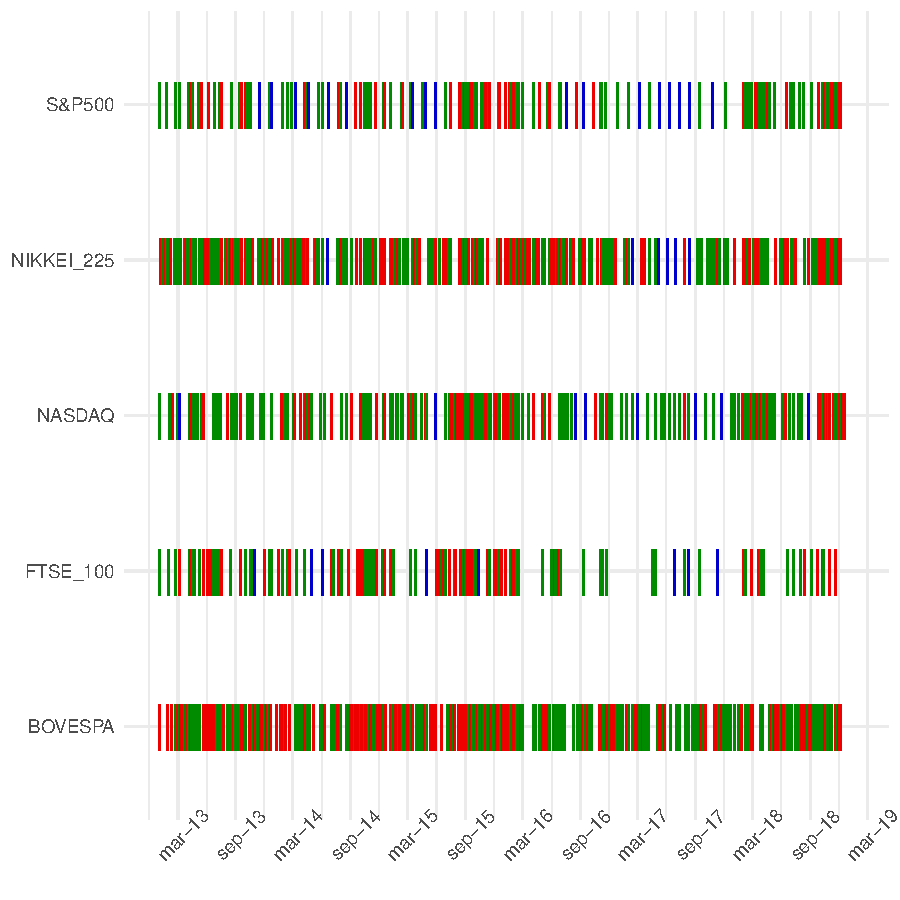
\includegraphics{main-029}
\caption{Clasificación de la simulación}
\end{figure}

Se observa como en la simulación utilizando el índice BOVESPA, los trades positivos aumentan su frecuencia a partir del segundo semestre del 2016, esto puede deberse al hecho de tener mayor número de observaciones para entrenar el modelo. Igualmente se aprecia como para el S\&P500 las operaciones se concentran en los primeros años de prueba, cerrando los demás años practicamente sin operaciones.


\begin{figure}[H]
\setkeys{Gin}{width = 1\textwidth}
\centering
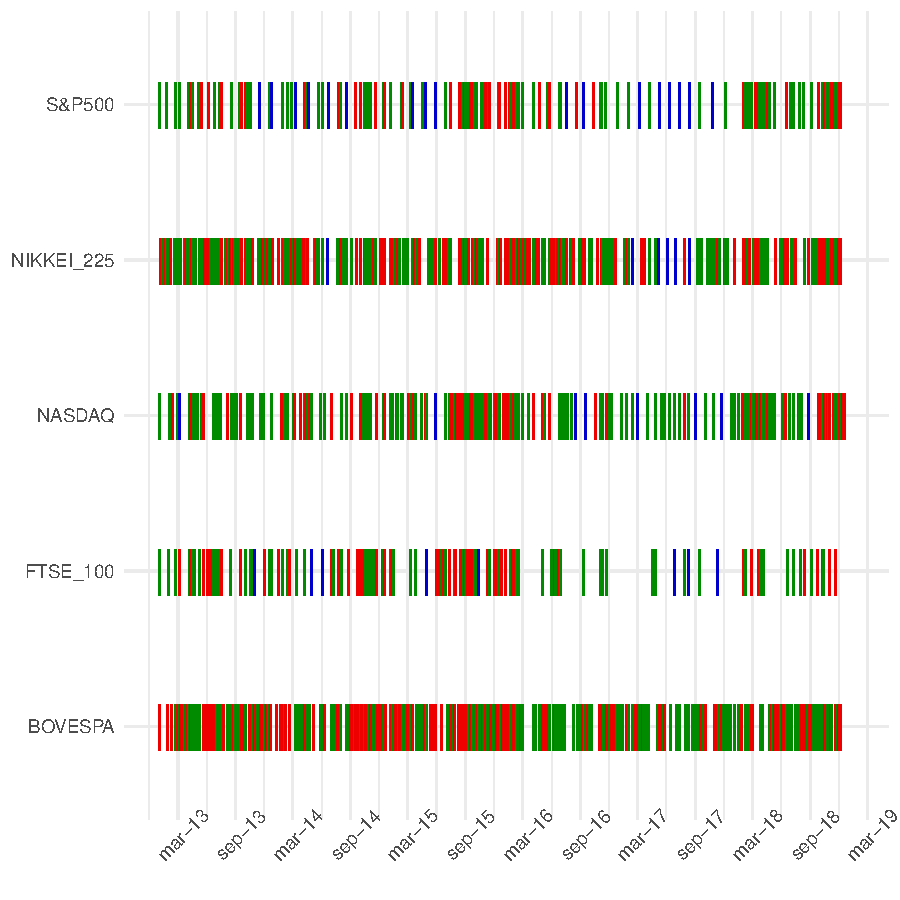
\includegraphics{main-031}
\caption{Retorno acumulado para cada índice}
\end{figure}

\subsection{Medidas de Riesgo}

Al asumir que siempre se abre la posición con la misma cantidad de dinero, en este caso 1000 USD, se sabe que los trades solo pueden arrojar dos resultados -0.02\% de ganancia en caso que sea positivo ó 0.025\% de pérdida en caso contrario, descartando las liquidaciones por límite de tiempo- En este sentido se aplica el contraste Wald–Wolfowitz comunmente llamado test de racha, para verificar la aleatoriedad de los resultados de los trades.

La prueba de Wald–Wolfowitz se puede definir de la siguiente manera:

\begin{itemize}
\item \textbf{H0}: La secuencia es producida de manera aleatoria.
\item \textbf{Hi}: La secuencia no es producida de manera aleatoria.
\end{itemize}

 
\begin{center}
\captionof{table}{Resultados del test de Wald–Wolfowitz (Test de Racha)}
% latex table generated in R 3.5.3 by xtable 1.8-3 package
% Thu Mar 14 23:34:01 2019
\begin{table}[ht]
\centering
\begin{tabular}{rrr}
  \hline
 & statistic & p.value \\ 
  \hline
S\&P\_500 & -0.83 & 0.41 \\ 
  NASDAQ & 0.16 & 0.87 \\ 
  NIKKEI\_225 & 1.19 & 0.23 \\ 
  FTSE\_100 & 1.09 & 0.28 \\ 
  BOVESPA & -0.09 & 0.93 \\ 
   \hline
\end{tabular}
\end{table}\end{center}

Frente a p-valores mayores a 0.05, y con un nivel de significación del 5\% no existen elementos suficientes para rechazar la hipótesis nula de aleatoriedad en la secuencia de los resultados de los trades, por lo que se puede concluir que los trades son independientes.

Asumiendo que la ocurrencia de los trades se distribuye de manera uniforme es posible modelar el retorno de capital y calcular VaR y ES para cada índice.


\begin{center}
\captionof{table}{VaR y ES para retornos de cada índice}
% latex table generated in R 3.5.3 by xtable 1.8-3 package
% Thu Mar 14 23:34:01 2019
\begin{table}[ht]
\centering
\begin{tabular}{rrrrrr}
  \hline
 & S\&P\_500 & NASDAQ & NIKKEI\_225 & FTSE\_100 & BOVESPA \\ 
  \hline
VaR & 1517.08 & 827.06 & 2362.36 & 2661.70 & 2366.74 \\ 
  ES & 1792.23 & 898.16 & 2947.89 & 3375.43 & 2954.07 \\ 
   \hline
\end{tabular}
\end{table}\end{center}
  
% !TeX root = ./main.Rnw
%\SweaveUTF8

\chapter*{Conclusiones y Recomendaciones}
\addcontentsline{toc}{chapter}{Conclusiones y Recomendaciones}

En esta investigación se ha planteado un marco de trabajo que permite el desarrollo y prueba para una estrategia de trading automatizado. En ningún momento se busca medir la posible ganancia en base a la simulación, sino, demostrar que es posible obtener rendimientos con una estrategia basada en indicadores técnicos utilizados como variables predictoras en un modelo de aprendizaje automático. En los resultados no se contemplan las comisiones acarreadas por la operación de los activo. Se asume también que siempre se logra comprar la cantidad establecida en el precio de cierre de la vela, hecho que no siempre ocurre sobre todo en mercados de alta volatilidad y poca liquidez.

Si bien el retorno acumulado durante 6 años de prueba es poco atractivo, los resultados de la precisión dejan ver la posibilidad de un amplio rango de mejora en el performance de la estrategia. Este modelo puede ser mejorado de muchas maneras, incluyendo, por ejemplo la optimización de los parámetros tp, sl y h para el activo a operar, así como la elección del tamaño de los períodos de entrenamiento. Otras de las limitaciones presente es el de utilizar un modelo lineal, si bien se decide utilizar MLG como punto de partida es muy probable que algún modelo que no asuma linealidad como árboles de decisíon o SVM mejoren la predicción. 

El modelo solo considera la prediccion del incremento del precio. Se utiliza la figura del stop loss como reduccion del riesgo. Un alternativa para obtener protección podría ser invertir el modelo, es decir predecir una disminución del precio, de esta manera se podría dejar de lado el stop loss y liquidar la posición cuando el modelo prediga una disminución en los precios.

Otra posible fuente de optimización podría ser la elección de los indicadores técnicos. Se podría profundizar en el aspecto técnico para su elección y el de las confifuraciones de los mismos buscando mejorar la predicción del modelo. De cualquier manera esta investigación busca ser un punto de partida para futuras investigaciones.


% !TeX root = ./main.Rnw
%\SweaveUTF8

\chapter{Anexos}

\section{Coeficientes de los modelos}

En la tabla 4.1 se describen los resultados de los parámetros arrojados por la regresión logística en los 6 períodos de entrenamiento para la serie del NASDAQ.
\begin{center}
\captionof{table}{Resumen del modelo para cada período de entrenamiento utilizando S\&P500}
\captionof*{table}{Período de entrenamiento 2009 - 2012}
% latex table generated in R 3.5.3 by xtable 1.8-3 package
% Thu Mar 14 23:34:01 2019
\begin{table}[ht]
\centering
\begin{tabular}{rrrrr}
  \hline
 & Estimate & Std. Error & z value & Pr($>$$|$z$|$) \\ 
  \hline
(Intercept) & -0.3153 & 0.0641 & -4.92 & 0.0000 \\ 
  PC1 & -0.0020 & 0.0181 & -0.11 & 0.9133 \\ 
  PC2 & 0.0055 & 0.0206 & 0.27 & 0.7905 \\ 
  PC3 & -0.0248 & 0.0316 & -0.79 & 0.4319 \\ 
  PC4 & -0.0245 & 0.0339 & -0.73 & 0.4684 \\ 
  PC5 & -0.0041 & 0.0369 & -0.11 & 0.9107 \\ 
  PC6 & -0.0903 & 0.0392 & -2.31 & 0.0212 \\ 
  PC7 & 0.0570 & 0.0449 & 1.27 & 0.2038 \\ 
   \hline
\end{tabular}
\end{table}\end{center}

\newpage
\begin{center}
\captionof*{table}{Período de entrenamiento 2009 - 2013}
% latex table generated in R 3.5.3 by xtable 1.8-3 package
% Thu Mar 14 23:34:01 2019
\begin{table}[ht]
\centering
\begin{tabular}{rrrrr}
  \hline
 & Estimate & Std. Error & z value & Pr($>$$|$z$|$) \\ 
  \hline
(Intercept) & -0.3669 & 0.0574 & -6.39 & 0.0000 \\ 
  PC1 & 0.0123 & 0.0164 & 0.75 & 0.4527 \\ 
  PC2 & -0.0000 & 0.0184 & -0.00 & 0.9992 \\ 
  PC3 & 0.0129 & 0.0280 & 0.46 & 0.6459 \\ 
  PC4 & -0.0142 & 0.0296 & -0.48 & 0.6313 \\ 
  PC5 & -0.0049 & 0.0316 & -0.16 & 0.8762 \\ 
  PC6 & 0.0084 & 0.0331 & 0.25 & 0.8005 \\ 
  PC7 & 0.0034 & 0.0394 & 0.09 & 0.9322 \\ 
   \hline
\end{tabular}
\end{table}\end{center}
\begin{center}
\captionof*{table}{Período de entrenamiento 2009 - 2014}
% latex table generated in R 3.5.3 by xtable 1.8-3 package
% Thu Mar 14 23:34:01 2019
\begin{table}[ht]
\centering
\begin{tabular}{rrrrr}
  \hline
 & Estimate & Std. Error & z value & Pr($>$$|$z$|$) \\ 
  \hline
(Intercept) & -0.3036 & 0.0522 & -5.81 & 0.0000 \\ 
  PC1 & 0.0291 & 0.0153 & 1.91 & 0.0564 \\ 
  PC2 & -0.0210 & 0.0172 & -1.22 & 0.2238 \\ 
  PC3 & 0.0341 & 0.0230 & 1.48 & 0.1390 \\ 
  PC4 & 0.0006 & 0.0263 & 0.02 & 0.9809 \\ 
  PC5 & 0.0062 & 0.0305 & 0.20 & 0.8392 \\ 
  PC6 & -0.0362 & 0.0314 & -1.15 & 0.2490 \\ 
  PC7 & 0.0169 & 0.0373 & 0.45 & 0.6505 \\ 
   \hline
\end{tabular}
\end{table}\end{center}
\begin{center}
\captionof*{table}{Período de entrenamiento 2009 - 2015}
% latex table generated in R 3.5.3 by xtable 1.8-3 package
% Thu Mar 14 23:34:01 2019
\begin{table}[ht]
\centering
\begin{tabular}{rrrrr}
  \hline
 & Estimate & Std. Error & z value & Pr($>$$|$z$|$) \\ 
  \hline
(Intercept) & -0.2767 & 0.0485 & -5.71 & 0.0000 \\ 
  PC1 & 0.0524 & 0.0148 & 3.55 & 0.0004 \\ 
  PC2 & -0.0257 & 0.0162 & -1.59 & 0.1123 \\ 
  PC3 & 0.0477 & 0.0207 & 2.31 & 0.0210 \\ 
  PC4 & -0.0027 & 0.0251 & -0.11 & 0.9137 \\ 
  PC5 & -0.0398 & 0.0287 & -1.39 & 0.1655 \\ 
  PC6 & -0.0424 & 0.0296 & -1.44 & 0.1511 \\ 
  PC7 & -0.0138 & 0.0353 & -0.39 & 0.6951 \\ 
   \hline
\end{tabular}
\end{table}\end{center}
\newpage
\begin{center}
\captionof*{table}{Período de entrenamiento 2009 - 2016}
% latex table generated in R 3.5.3 by xtable 1.8-3 package
% Thu Mar 14 23:34:01 2019
\begin{table}[ht]
\centering
\begin{tabular}{rrrrr}
  \hline
 & Estimate & Std. Error & z value & Pr($>$$|$z$|$) \\ 
  \hline
(Intercept) & -0.2653 & 0.0452 & -5.86 & 0.0000 \\ 
  PC1 & -0.0421 & 0.0135 & -3.12 & 0.0018 \\ 
  PC2 & 0.0301 & 0.0150 & 2.01 & 0.0448 \\ 
  PC3 & 0.0527 & 0.0192 & 2.74 & 0.0062 \\ 
  PC4 & -0.0023 & 0.0231 & -0.10 & 0.9223 \\ 
  PC5 & -0.0131 & 0.0265 & -0.49 & 0.6219 \\ 
  PC6 & -0.0302 & 0.0282 & -1.07 & 0.2839 \\ 
  PC7 & -0.0084 & 0.0328 & -0.25 & 0.7990 \\ 
   \hline
\end{tabular}
\end{table}\end{center}
\begin{center}
\captionof*{table}{Período de entrenamiento 2009 - 2017}
% latex table generated in R 3.5.3 by xtable 1.8-3 package
% Thu Mar 14 23:34:01 2019
\begin{table}[ht]
\centering
\begin{tabular}{rrrrr}
  \hline
 & Estimate & Std. Error & z value & Pr($>$$|$z$|$) \\ 
  \hline
(Intercept) & -0.3421 & 0.0428 & -7.99 & 0.0000 \\ 
  PC1 & 0.0352 & 0.0128 & 2.75 & 0.0059 \\ 
  PC2 & -0.0316 & 0.0142 & -2.23 & 0.0257 \\ 
  PC3 & -0.0096 & 0.0178 & -0.54 & 0.5888 \\ 
  PC4 & -0.0227 & 0.0213 & -1.06 & 0.2870 \\ 
  PC5 & -0.0062 & 0.0250 & -0.25 & 0.8053 \\ 
  PC6 & 0.0388 & 0.0260 & 1.49 & 0.1358 \\ 
  PC7 & 0.0225 & 0.0306 & 0.74 & 0.4613 \\ 
   \hline
\end{tabular}
\end{table}\end{center}


En la tabla 4.1 se describen los resultados de los parámetros arrojados por la regresión logística en los 6 períodos de entrenamiento para la serie del NIKKEI 225.
\begin{center}
\captionof{table}{Resumen del modelo para cada período de entrenamiento utilizando S\&P500}
\captionof*{table}{Período de entrenamiento 2009 - 2012}
% latex table generated in R 3.5.3 by xtable 1.8-3 package
% Thu Mar 14 23:34:01 2019
\begin{table}[ht]
\centering
\begin{tabular}{rrrrr}
  \hline
 & Estimate & Std. Error & z value & Pr($>$$|$z$|$) \\ 
  \hline
(Intercept) & -0.2578 & 0.0650 & -3.96 & 0.0001 \\ 
  PC1 & -0.0159 & 0.0181 & -0.88 & 0.3796 \\ 
  PC2 & -0.0238 & 0.0229 & -1.04 & 0.2989 \\ 
  PC3 & -0.0435 & 0.0310 & -1.40 & 0.1605 \\ 
  PC4 & 0.0308 & 0.0370 & 0.83 & 0.4053 \\ 
  PC5 & -0.0809 & 0.0413 & -1.96 & 0.0504 \\ 
  PC6 & -0.0728 & 0.0434 & -1.68 & 0.0933 \\ 
  PC7 & -0.1040 & 0.0556 & -1.87 & 0.0614 \\ 
   \hline
\end{tabular}
\end{table}\end{center}

\newpage
\begin{center}
\captionof*{table}{Período de entrenamiento 2009 - 2013}
% latex table generated in R 3.5.3 by xtable 1.8-3 package
% Thu Mar 14 23:34:01 2019
\begin{table}[ht]
\centering
\begin{tabular}{rrrrr}
  \hline
 & Estimate & Std. Error & z value & Pr($>$$|$z$|$) \\ 
  \hline
(Intercept) & -0.3339 & 0.0585 & -5.71 & 0.0000 \\ 
  PC1 & -0.0259 & 0.0159 & -1.63 & 0.1035 \\ 
  PC2 & -0.0098 & 0.0206 & -0.47 & 0.6364 \\ 
  PC3 & -0.0463 & 0.0284 & -1.63 & 0.1027 \\ 
  PC4 & -0.0377 & 0.0326 & -1.16 & 0.2478 \\ 
  PC5 & -0.1228 & 0.0379 & -3.24 & 0.0012 \\ 
  PC6 & -0.0380 & 0.0391 & -0.97 & 0.3322 \\ 
  PC7 & -0.0256 & 0.0473 & -0.54 & 0.5875 \\ 
   \hline
\end{tabular}
\end{table}\end{center}
\begin{center}
\captionof*{table}{Período de entrenamiento 2009 - 2014}
% latex table generated in R 3.5.3 by xtable 1.8-3 package
% Thu Mar 14 23:34:01 2019
\begin{table}[ht]
\centering
\begin{tabular}{rrrrr}
  \hline
 & Estimate & Std. Error & z value & Pr($>$$|$z$|$) \\ 
  \hline
(Intercept) & -0.3361 & 0.0533 & -6.30 & 0.0000 \\ 
  PC1 & -0.0148 & 0.0147 & -1.01 & 0.3126 \\ 
  PC2 & -0.0109 & 0.0185 & -0.59 & 0.5550 \\ 
  PC3 & -0.0226 & 0.0254 & -0.89 & 0.3730 \\ 
  PC4 & -0.0641 & 0.0302 & -2.12 & 0.0340 \\ 
  PC5 & -0.0969 & 0.0339 & -2.86 & 0.0042 \\ 
  PC6 & -0.0484 & 0.0360 & -1.34 & 0.1792 \\ 
  PC7 & -0.0357 & 0.0415 & -0.86 & 0.3898 \\ 
   \hline
\end{tabular}
\end{table}\end{center}
\begin{center}
\captionof*{table}{Período de entrenamiento 2009 - 2015}
% latex table generated in R 3.5.3 by xtable 1.8-3 package
% Thu Mar 14 23:34:01 2019
\begin{table}[ht]
\centering
\begin{tabular}{rrrrr}
  \hline
 & Estimate & Std. Error & z value & Pr($>$$|$z$|$) \\ 
  \hline
(Intercept) & -0.3076 & 0.0491 & -6.26 & 0.0000 \\ 
  PC1 & 0.0006 & 0.0140 & 0.04 & 0.9680 \\ 
  PC2 & -0.0062 & 0.0172 & -0.36 & 0.7162 \\ 
  PC3 & 0.0035 & 0.0207 & 0.17 & 0.8670 \\ 
  PC4 & -0.0645 & 0.0263 & -2.45 & 0.0143 \\ 
  PC5 & -0.0589 & 0.0302 & -1.95 & 0.0509 \\ 
  PC6 & -0.0345 & 0.0328 & -1.05 & 0.2938 \\ 
  PC7 & -0.0558 & 0.0381 & -1.47 & 0.1424 \\ 
   \hline
\end{tabular}
\end{table}\end{center}
\newpage
\begin{center}
\captionof*{table}{Período de entrenamiento 2009 - 2016}
% latex table generated in R 3.5.3 by xtable 1.8-3 package
% Thu Mar 14 23:34:01 2019
\begin{table}[ht]
\centering
\begin{tabular}{rrrrr}
  \hline
 & Estimate & Std. Error & z value & Pr($>$$|$z$|$) \\ 
  \hline
(Intercept) & -0.2862 & 0.0459 & -6.24 & 0.0000 \\ 
  PC1 & 0.0107 & 0.0134 & 0.80 & 0.4221 \\ 
  PC2 & -0.0055 & 0.0158 & -0.35 & 0.7268 \\ 
  PC3 & 0.0031 & 0.0191 & 0.16 & 0.8709 \\ 
  PC4 & 0.0659 & 0.0240 & 2.74 & 0.0061 \\ 
  PC5 & -0.0204 & 0.0270 & -0.76 & 0.4494 \\ 
  PC6 & -0.0488 & 0.0293 & -1.67 & 0.0958 \\ 
  PC7 & 0.0564 & 0.0362 & 1.56 & 0.1191 \\ 
   \hline
\end{tabular}
\end{table}\end{center}
\begin{center}
\captionof*{table}{Período de entrenamiento 2009 - 2017}
% latex table generated in R 3.5.3 by xtable 1.8-3 package
% Thu Mar 14 23:34:01 2019
\begin{table}[ht]
\centering
\begin{tabular}{rrrrr}
  \hline
 & Estimate & Std. Error & z value & Pr($>$$|$z$|$) \\ 
  \hline
(Intercept) & -0.2769 & 0.0430 & -6.44 & 0.0000 \\ 
  PC1 & 0.0010 & 0.0125 & 0.08 & 0.9348 \\ 
  PC2 & 0.0031 & 0.0150 & 0.21 & 0.8353 \\ 
  PC3 & -0.0264 & 0.0188 & -1.41 & 0.1592 \\ 
  PC4 & 0.0533 & 0.0226 & 2.35 & 0.0186 \\ 
  PC5 & -0.0141 & 0.0255 & -0.55 & 0.5794 \\ 
  PC6 & 0.0960 & 0.0308 & 3.12 & 0.0018 \\ 
  PC7 & -0.0452 & 0.0315 & -1.44 & 0.1510 \\ 
   \hline
\end{tabular}
\end{table}\end{center}



En la tabla 4.1 se describen los resultados de los parámetros arrojados por la regresión logística en los 6 períodos de entrenamiento para la serie del FTSE 100.
\begin{center}
\captionof{table}{Resumen del modelo para cada período de entrenamiento utilizando S\&P500}
\captionof*{table}{Período de entrenamiento 2009 - 2012}
% latex table generated in R 3.5.3 by xtable 1.8-3 package
% Thu Mar 14 23:34:01 2019
\begin{table}[ht]
\centering
\begin{tabular}{rrrrr}
  \hline
 & Estimate & Std. Error & z value & Pr($>$$|$z$|$) \\ 
  \hline
(Intercept) & -0.1552 & 0.0636 & -2.44 & 0.0147 \\ 
  PC1 & -0.0386 & 0.0182 & -2.12 & 0.0343 \\ 
  PC2 & -0.0074 & 0.0208 & -0.36 & 0.7207 \\ 
  PC3 & -0.0355 & 0.0306 & -1.16 & 0.2467 \\ 
  PC4 & 0.0327 & 0.0361 & 0.91 & 0.3643 \\ 
  PC5 & -0.0481 & 0.0364 & -1.32 & 0.1859 \\ 
  PC6 & 0.0770 & 0.0429 & 1.79 & 0.0731 \\ 
  PC7 & -0.0519 & 0.0509 & -1.02 & 0.3071 \\ 
   \hline
\end{tabular}
\end{table}\end{center}

\newpage
\begin{center}
\captionof*{table}{Período de entrenamiento 2009 - 2013}
% latex table generated in R 3.5.3 by xtable 1.8-3 package
% Thu Mar 14 23:34:01 2019
\begin{table}[ht]
\centering
\begin{tabular}{rrrrr}
  \hline
 & Estimate & Std. Error & z value & Pr($>$$|$z$|$) \\ 
  \hline
(Intercept) & -0.1569 & 0.0568 & -2.76 & 0.0057 \\ 
  PC1 & 0.0402 & 0.0164 & 2.45 & 0.0142 \\ 
  PC2 & 0.0237 & 0.0186 & 1.28 & 0.2017 \\ 
  PC3 & -0.0240 & 0.0281 & -0.85 & 0.3938 \\ 
  PC4 & 0.0090 & 0.0312 & 0.29 & 0.7722 \\ 
  PC5 & -0.0282 & 0.0325 & -0.87 & 0.3863 \\ 
  PC6 & 0.0237 & 0.0357 & 0.66 & 0.5077 \\ 
  PC7 & -0.0446 & 0.0453 & -0.98 & 0.3253 \\ 
   \hline
\end{tabular}
\end{table}\end{center}
\begin{center}
\captionof*{table}{Período de entrenamiento 2009 - 2014}
% latex table generated in R 3.5.3 by xtable 1.8-3 package
% Thu Mar 14 23:34:01 2019
\begin{table}[ht]
\centering
\begin{tabular}{rrrrr}
  \hline
 & Estimate & Std. Error & z value & Pr($>$$|$z$|$) \\ 
  \hline
(Intercept) & -0.0439 & 0.0522 & -0.84 & 0.4007 \\ 
  PC1 & -0.0597 & 0.0155 & -3.85 & 0.0001 \\ 
  PC2 & -0.0513 & 0.0177 & -2.90 & 0.0037 \\ 
  PC3 & -0.0617 & 0.0266 & -2.32 & 0.0204 \\ 
  PC4 & 0.0001 & 0.0290 & 0.00 & 0.9980 \\ 
  PC5 & -0.0624 & 0.0308 & -2.03 & 0.0425 \\ 
  PC6 & 0.0899 & 0.0326 & 2.75 & 0.0059 \\ 
  PC7 & 0.0054 & 0.0424 & 0.13 & 0.8989 \\ 
   \hline
\end{tabular}
\end{table}\end{center}
\begin{center}
\captionof*{table}{Período de entrenamiento 2009 - 2015}
% latex table generated in R 3.5.3 by xtable 1.8-3 package
% Thu Mar 14 23:34:01 2019
\begin{table}[ht]
\centering
\begin{tabular}{rrrrr}
  \hline
 & Estimate & Std. Error & z value & Pr($>$$|$z$|$) \\ 
  \hline
(Intercept) & 0.0397 & 0.0486 & 0.82 & 0.4137 \\ 
  PC1 & -0.0790 & 0.0151 & -5.25 & 0.0000 \\ 
  PC2 & -0.0381 & 0.0163 & -2.34 & 0.0192 \\ 
  PC3 & 0.0688 & 0.0263 & 2.62 & 0.0088 \\ 
  PC4 & -0.0075 & 0.0283 & -0.26 & 0.7920 \\ 
  PC5 & -0.0187 & 0.0285 & -0.66 & 0.5111 \\ 
  PC6 & 0.1536 & 0.0327 & 4.70 & 0.0000 \\ 
  PC7 & -0.0560 & 0.0422 & -1.33 & 0.1849 \\ 
   \hline
\end{tabular}
\end{table}\end{center}
\newpage
\begin{center}
\captionof*{table}{Período de entrenamiento 2009 - 2016}
% latex table generated in R 3.5.3 by xtable 1.8-3 package
% Thu Mar 14 23:34:01 2019
\begin{table}[ht]
\centering
\begin{tabular}{rrrrr}
  \hline
 & Estimate & Std. Error & z value & Pr($>$$|$z$|$) \\ 
  \hline
(Intercept) & -0.0231 & 0.0454 & -0.51 & 0.6110 \\ 
  PC1 & -0.0713 & 0.0140 & -5.09 & 0.0000 \\ 
  PC2 & -0.0478 & 0.0156 & -3.07 & 0.0021 \\ 
  PC3 & 0.0664 & 0.0248 & 2.68 & 0.0073 \\ 
  PC4 & 0.0020 & 0.0261 & 0.08 & 0.9378 \\ 
  PC5 & -0.0181 & 0.0268 & -0.67 & 0.5005 \\ 
  PC6 & 0.1481 & 0.0315 & 4.70 & 0.0000 \\ 
  PC7 & -0.0981 & 0.0354 & -2.77 & 0.0055 \\ 
   \hline
\end{tabular}
\end{table}\end{center}
\begin{center}
\captionof*{table}{Período de entrenamiento 2009 - 2017}
% latex table generated in R 3.5.3 by xtable 1.8-3 package
% Thu Mar 14 23:34:01 2019
\begin{table}[ht]
\centering
\begin{tabular}{rrrrr}
  \hline
 & Estimate & Std. Error & z value & Pr($>$$|$z$|$) \\ 
  \hline
(Intercept) & 0.0301 & 0.0429 & 0.70 & 0.4821 \\ 
  PC1 & -0.0784 & 0.0134 & -5.87 & 0.0000 \\ 
  PC2 & -0.0546 & 0.0147 & -3.73 & 0.0002 \\ 
  PC3 & 0.0659 & 0.0232 & 2.84 & 0.0045 \\ 
  PC4 & -0.0188 & 0.0245 & -0.77 & 0.4416 \\ 
  PC5 & -0.0139 & 0.0253 & -0.55 & 0.5841 \\ 
  PC6 & 0.1413 & 0.0280 & 5.05 & 0.0000 \\ 
  PC7 & -0.0374 & 0.0361 & -1.04 & 0.2997 \\ 
   \hline
\end{tabular}
\end{table}\end{center}



En la tabla 4.1 se describen los resultados de los parámetros arrojados por la regresión logística en los 6 períodos de entrenamiento para la serie del BOVESPA.
\begin{center}
\captionof{table}{Resumen del modelo para cada período de entrenamiento utilizando S\&P500}
\captionof*{table}{Período de entrenamiento 2009 - 2012}
% latex table generated in R 3.5.3 by xtable 1.8-3 package
% Thu Mar 14 23:34:01 2019
\begin{table}[ht]
\centering
\begin{tabular}{rrrrr}
  \hline
 & Estimate & Std. Error & z value & Pr($>$$|$z$|$) \\ 
  \hline
(Intercept) & -0.2445 & 0.0646 & -3.78 & 0.0002 \\ 
  PC1 & -0.0190 & 0.0177 & -1.07 & 0.2835 \\ 
  PC2 & -0.0090 & 0.0223 & -0.40 & 0.6878 \\ 
  PC3 & 0.0169 & 0.0293 & 0.58 & 0.5637 \\ 
  PC4 & -0.0675 & 0.0325 & -2.08 & 0.0380 \\ 
  PC5 & 0.0081 & 0.0387 & 0.21 & 0.8344 \\ 
  PC6 & 0.0929 & 0.0433 & 2.14 & 0.0320 \\ 
  PC7 & -0.0947 & 0.0450 & -2.11 & 0.0351 \\ 
   \hline
\end{tabular}
\end{table}\end{center}

\newpage
\begin{center}
\captionof*{table}{Período de entrenamiento 2009 - 2013}
% latex table generated in R 3.5.3 by xtable 1.8-3 package
% Thu Mar 14 23:34:01 2019
\begin{table}[ht]
\centering
\begin{tabular}{rrrrr}
  \hline
 & Estimate & Std. Error & z value & Pr($>$$|$z$|$) \\ 
  \hline
(Intercept) & -0.1524 & 0.0574 & -2.66 & 0.0079 \\ 
  PC1 & -0.0158 & 0.0158 & -1.00 & 0.3179 \\ 
  PC2 & -0.0183 & 0.0201 & -0.91 & 0.3640 \\ 
  PC3 & 0.0306 & 0.0274 & 1.12 & 0.2635 \\ 
  PC4 & -0.0373 & 0.0293 & -1.27 & 0.2029 \\ 
  PC5 & 0.0233 & 0.0346 & 0.68 & 0.4993 \\ 
  PC6 & 0.0196 & 0.0378 & 0.52 & 0.6038 \\ 
  PC7 & 0.1188 & 0.0416 & 2.86 & 0.0043 \\ 
   \hline
\end{tabular}
\end{table}\end{center}
\begin{center}
\captionof*{table}{Período de entrenamiento 2009 - 2014}
% latex table generated in R 3.5.3 by xtable 1.8-3 package
% Thu Mar 14 23:34:01 2019
\begin{table}[ht]
\centering
\begin{tabular}{rrrrr}
  \hline
 & Estimate & Std. Error & z value & Pr($>$$|$z$|$) \\ 
  \hline
(Intercept) & -0.1078 & 0.0520 & -2.07 & 0.0380 \\ 
  PC1 & -0.0138 & 0.0144 & -0.95 & 0.3399 \\ 
  PC2 & -0.0185 & 0.0179 & -1.04 & 0.3004 \\ 
  PC3 & 0.0276 & 0.0248 & 1.11 & 0.2660 \\ 
  PC4 & -0.0498 & 0.0264 & -1.88 & 0.0597 \\ 
  PC5 & 0.0108 & 0.0311 & 0.35 & 0.7284 \\ 
  PC6 & 0.0147 & 0.0328 & 0.45 & 0.6529 \\ 
  PC7 & 0.0979 & 0.0376 & 2.61 & 0.0092 \\ 
   \hline
\end{tabular}
\end{table}\end{center}
\begin{center}
\captionof*{table}{Período de entrenamiento 2009 - 2015}
% latex table generated in R 3.5.3 by xtable 1.8-3 package
% Thu Mar 14 23:34:01 2019
\begin{table}[ht]
\centering
\begin{tabular}{rrrrr}
  \hline
 & Estimate & Std. Error & z value & Pr($>$$|$z$|$) \\ 
  \hline
(Intercept) & -0.0762 & 0.0479 & -1.59 & 0.1122 \\ 
  PC1 & 0.0127 & 0.0133 & 0.96 & 0.3382 \\ 
  PC2 & -0.0097 & 0.0165 & -0.59 & 0.5559 \\ 
  PC3 & -0.0329 & 0.0230 & -1.43 & 0.1516 \\ 
  PC4 & 0.0445 & 0.0242 & 1.84 & 0.0657 \\ 
  PC5 & 0.0032 & 0.0286 & 0.11 & 0.9096 \\ 
  PC6 & -0.0450 & 0.0306 & -1.47 & 0.1410 \\ 
  PC7 & 0.0768 & 0.0351 & 2.19 & 0.0288 \\ 
   \hline
\end{tabular}
\end{table}\end{center}
\newpage
\begin{center}
\captionof*{table}{Período de entrenamiento 2009 - 2016}
% latex table generated in R 3.5.3 by xtable 1.8-3 package
% Thu Mar 14 23:34:01 2019
\begin{table}[ht]
\centering
\begin{tabular}{rrrrr}
  \hline
 & Estimate & Std. Error & z value & Pr($>$$|$z$|$) \\ 
  \hline
(Intercept) & -0.1270 & 0.0448 & -2.83 & 0.0046 \\ 
  PC1 & 0.0098 & 0.0122 & 0.80 & 0.4227 \\ 
  PC2 & -0.0063 & 0.0156 & -0.41 & 0.6848 \\ 
  PC3 & -0.0143 & 0.0210 & -0.68 & 0.4970 \\ 
  PC4 & 0.0314 & 0.0225 & 1.40 & 0.1625 \\ 
  PC5 & 0.0064 & 0.0268 & 0.24 & 0.8101 \\ 
  PC6 & -0.0206 & 0.0280 & -0.73 & 0.4625 \\ 
  PC7 & 0.0827 & 0.0324 & 2.56 & 0.0106 \\ 
   \hline
\end{tabular}
\end{table}\end{center}
\begin{center}
\captionof*{table}{Período de entrenamiento 2009 - 2017}
% latex table generated in R 3.5.3 by xtable 1.8-3 package
% Thu Mar 14 23:34:01 2019
\begin{table}[ht]
\centering
\begin{tabular}{rrrrr}
  \hline
 & Estimate & Std. Error & z value & Pr($>$$|$z$|$) \\ 
  \hline
(Intercept) & -0.1857 & 0.0424 & -4.38 & 0.0000 \\ 
  PC1 & 0.0068 & 0.0114 & 0.60 & 0.5492 \\ 
  PC2 & -0.0043 & 0.0147 & -0.29 & 0.7718 \\ 
  PC3 & -0.0149 & 0.0198 & -0.75 & 0.4536 \\ 
  PC4 & 0.0156 & 0.0211 & 0.74 & 0.4607 \\ 
  PC5 & 0.0042 & 0.0252 & 0.17 & 0.8672 \\ 
  PC6 & 0.0144 & 0.0268 & 0.54 & 0.5905 \\ 
  PC7 & 0.0517 & 0.0297 & 1.74 & 0.0818 \\ 
   \hline
\end{tabular}
\end{table}\end{center}

% !TeX root = ./main.Rnw
%\SweaveUTF8

\chapter*{Lista de Referencias}
\addcontentsline{toc}{chapter}{Lista de Referencias}

\begin{itemize}

\item Lu Ning (2016). \textit{A machine Learning Approach to Automated Trading}. USA, Coston College Computer Science.

\item Huertas López Alejandro (2015). \textit{Modelos Predictivos para el mercado FOREX}. España, Universidad de Murcia.

\item Shagilla Kadida Ramadhani (2006). \textit{Ab Analysis of Technical Trading Strategies}. Inglaterra, Leeds University Business School.

\item Bach William y Nielsen Kasper (2018). \textit{On Machine Learning Based Cryptocurrency Trading}. Dinamarca, Aalborg University.

\item Araneda Hugo (2015). \textit{Diseño e Implementación de un Sistema Automatizado Para Operar en el Mercado de Divisas Usando Reglas de Asociación}. Chile, Universidad de Chile.

\item Fernández Cristián (2008). \textit{Modelos Ocultos de Markov Aplicados al Reconocimiento de PAtrones del Análisis Técnico Búrsatil}. Argentina, Universidad Nacional de Córdoba.

\item James Gareth, Witten Daniela, Hastie Trevor y Tibshirani Robert (2013). \textit{An Introduction to Statistical Learning}. Springer.

\item Abhijit Ghatak (2017). \textit{Machine Learning with R}. Springer.

\item Murphy, J.J. (1999). \textit{Análisis Técnico de los Mercados Financieros}. New York Institute of Finance. New York: Gestión 2000.

\end{itemize}

\end{document}
